% Slides for talk on hydrogen fuel cells
% given in the department on October 27, 2003.
% 
% The original slides were in Prosper.  This file contains the
% translation of the original slides to Beamer.
% 
% Rouben Rostamian <rostamian@umbc.edu>
% August 31, 2004

\documentclass[10pt]{beamer}\usepackage[]{graphicx}\usepackage[]{xcolor}
% maxwidth is the original width if it is less than linewidth
% otherwise use linewidth (to make sure the graphics do not exceed the margin)
\makeatletter
\def\maxwidth{ %
  \ifdim\Gin@nat@width>\linewidth
    \linewidth
  \else
    \Gin@nat@width
  \fi
}
\makeatother

\definecolor{fgcolor}{rgb}{0.345, 0.345, 0.345}
\newcommand{\hlnum}[1]{\textcolor[rgb]{0.686,0.059,0.569}{#1}}%
\newcommand{\hlstr}[1]{\textcolor[rgb]{0.192,0.494,0.8}{#1}}%
\newcommand{\hlcom}[1]{\textcolor[rgb]{0.678,0.584,0.686}{\textit{#1}}}%
\newcommand{\hlopt}[1]{\textcolor[rgb]{0,0,0}{#1}}%
\newcommand{\hlstd}[1]{\textcolor[rgb]{0.345,0.345,0.345}{#1}}%
\newcommand{\hlkwa}[1]{\textcolor[rgb]{0.161,0.373,0.58}{\textbf{#1}}}%
\newcommand{\hlkwb}[1]{\textcolor[rgb]{0.69,0.353,0.396}{#1}}%
\newcommand{\hlkwc}[1]{\textcolor[rgb]{0.333,0.667,0.333}{#1}}%
\newcommand{\hlkwd}[1]{\textcolor[rgb]{0.737,0.353,0.396}{\textbf{#1}}}%
\let\hlipl\hlkwb

\usepackage{framed}
\makeatletter
\newenvironment{kframe}{%
 \def\at@end@of@kframe{}%
 \ifinner\ifhmode%
  \def\at@end@of@kframe{\end{minipage}}%
  \begin{minipage}{\columnwidth}%
 \fi\fi%
 \def\FrameCommand##1{\hskip\@totalleftmargin \hskip-\fboxsep
 \colorbox{shadecolor}{##1}\hskip-\fboxsep
     % There is no \\@totalrightmargin, so:
     \hskip-\linewidth \hskip-\@totalleftmargin \hskip\columnwidth}%
 \MakeFramed {\advance\hsize-\width
   \@totalleftmargin\z@ \linewidth\hsize
   \@setminipage}}%
 {\par\unskip\endMakeFramed%
 \at@end@of@kframe}
\makeatother

\definecolor{shadecolor}{rgb}{.97, .97, .97}
\definecolor{messagecolor}{rgb}{0, 0, 0}
\definecolor{warningcolor}{rgb}{1, 0, 1}
\definecolor{errorcolor}{rgb}{1, 0, 0}
\newenvironment{knitrout}{}{} % an empty environment to be redefined in TeX

\usepackage{alltt}
\usetheme{umbc4}
\usepackage{tikz}
\usepackage{colortbl}
\usepackage[absolute,overlay]{textpos}
%\usepackage{movie15}
\usepackage{multimedia}
\useinnertheme{umbcboxes}
\setbeamercolor{umbcboxes}{bg=violet!12,fg=black}
\usepackage{synttree}
\usepackage{multirow}
\usepackage{amsmath}



\usepackage{rotating} % for defining \schwa

\newcommand{\pop}[1]{{\textcolor{red}{#1}}}
\newcommand{\schwa}{\raisebox{1ex}{\begin{turn}{180}e\end{turn}}}
\newcommand{\death}[1]{{\textcolor{white}{#1}}}
\newcommand{\mob}[1]{{\textcolor{black}{#1}}}
\definecolor{darkblue}{rgb}{.3,0,.7}
\newcommand{\darkblue}[1]{{\textcolor{darkblue}{#1}}}
\newcommand{\birth}[1]{{\textcolor{white}{#1}}}

\definecolor{blue}{rgb}{0,0,1}
\newcommand{\blue}[1]{{\textcolor{blue}{#1}}}


%%%%%%%%
%%Bib
%%%%%%%%
\renewcommand{\refname}{}
\usepackage{natbib}
\usepackage{enumerate}

%%%%%%%%
%% Commands
%%%%%%%%
%in the definition of a new command you cannot use numbers
%see page 192 of Lamport
\newcommand{\ypop}{y=(y_1,y_2,\ldots,y_N)}
\newcommand{\ytot}{\sum_{i=1}^N y_i}
\newcommand{\ymn}{\sum_{i=1}^N y_i/N}
\newcommand{\ypva}{\sigma^2(y)}
\newcommand{\ypvb}{\sum_{i=1}^N(y_i - \bar{Y})^2/(N-1)}
\newcommand{\ysma}{y_{smp}}
\newcommand{\ysmb}{\{y_i\,:\,i\in smp\}}
\newcommand{\ybara}{\bar{y}_{smp}}
\newcommand{\ybarb}{\sum_{i \in smp} y_i/n}

\newcommand{\fred}{x+y=2}
\newcommand{\sally}[1]{x+y=#1}
\newcommand{\bill}[2]{x+ #1=#2}

%%% Local Variables: 
%%% mode: latex
%%% TeX-master: t
%%% End: 


\newcommand{\arcsinh}{\mathop\mathrm{arcsinh}\nolimits}
\newcommand{\arccosh}{\mathop\mathrm{arccosh}\nolimits}
\newcommand{\Pu}{P_{\mathrm{amb}}}
\DeclareMathOperator{\pr}{Pr}
%%%%%%%%
%% Commands
%%%%%%%%

%%%%%%%%
%% Block
%%%%%%%%
\definecolor{light-gray}{gray}{0.8}
\definecolor{lightskyblue}{rgb}{0.53,0.81,0.98}
\setbeamertemplate{blocks}[rounded][shadow=true]
\setbeamercolor{block title}{bg = gray, fg=white}
\setbeamercolor{block body}{bg = lightgray,fg=black}
\setbeamercolor{block body alerted}{bg = lightskyblue, fg=black}
\setbeamercolor{block tile alerted}{bg = lightskyblue, fg=black}
%%%%%%%%
%%blcok
%%%%%%%%


%%%%%%%%
%% itemize
%%%%%%%%
\definecolor{darkred}{rgb}{.8,0,0}  
\newcommand{\dd}[1]{{\textcolor{darkred}{#1}}}
\definecolor{lightblue}{rgb}{.2,0,1}  
\setbeamertemplate{itemize        item}{\large{\textcolor{darkred}{$\bullet$}}}
\setbeamertemplate{itemize     subitem}{\textcolor{lightblue}{$\bullet$}}
\setbeamertemplate{itemize  subsubitem}{$\bullet$}
%%%%%%%%
%% itemize
%%%%%%%%
%Network Dynamics:Distributional and Relationship Properties of Human Aggregates

\title[]{Survey Sampling One Day Course}
%\subtitle[]{}
\author[Zack W Almquist]{Zack W Almquist\\}
\institute[Department of Sociology,\\ University of Washington]{
  Department of Sociology\\
  University of Washington}
\date{Center for Statistics and the Social Sciences}
\IfFileExists{upquote.sty}{\usepackage{upquote}}{}
\begin{document}

%----------- titlepage ----------------------------------------------%
{
\usebackgroundtemplate{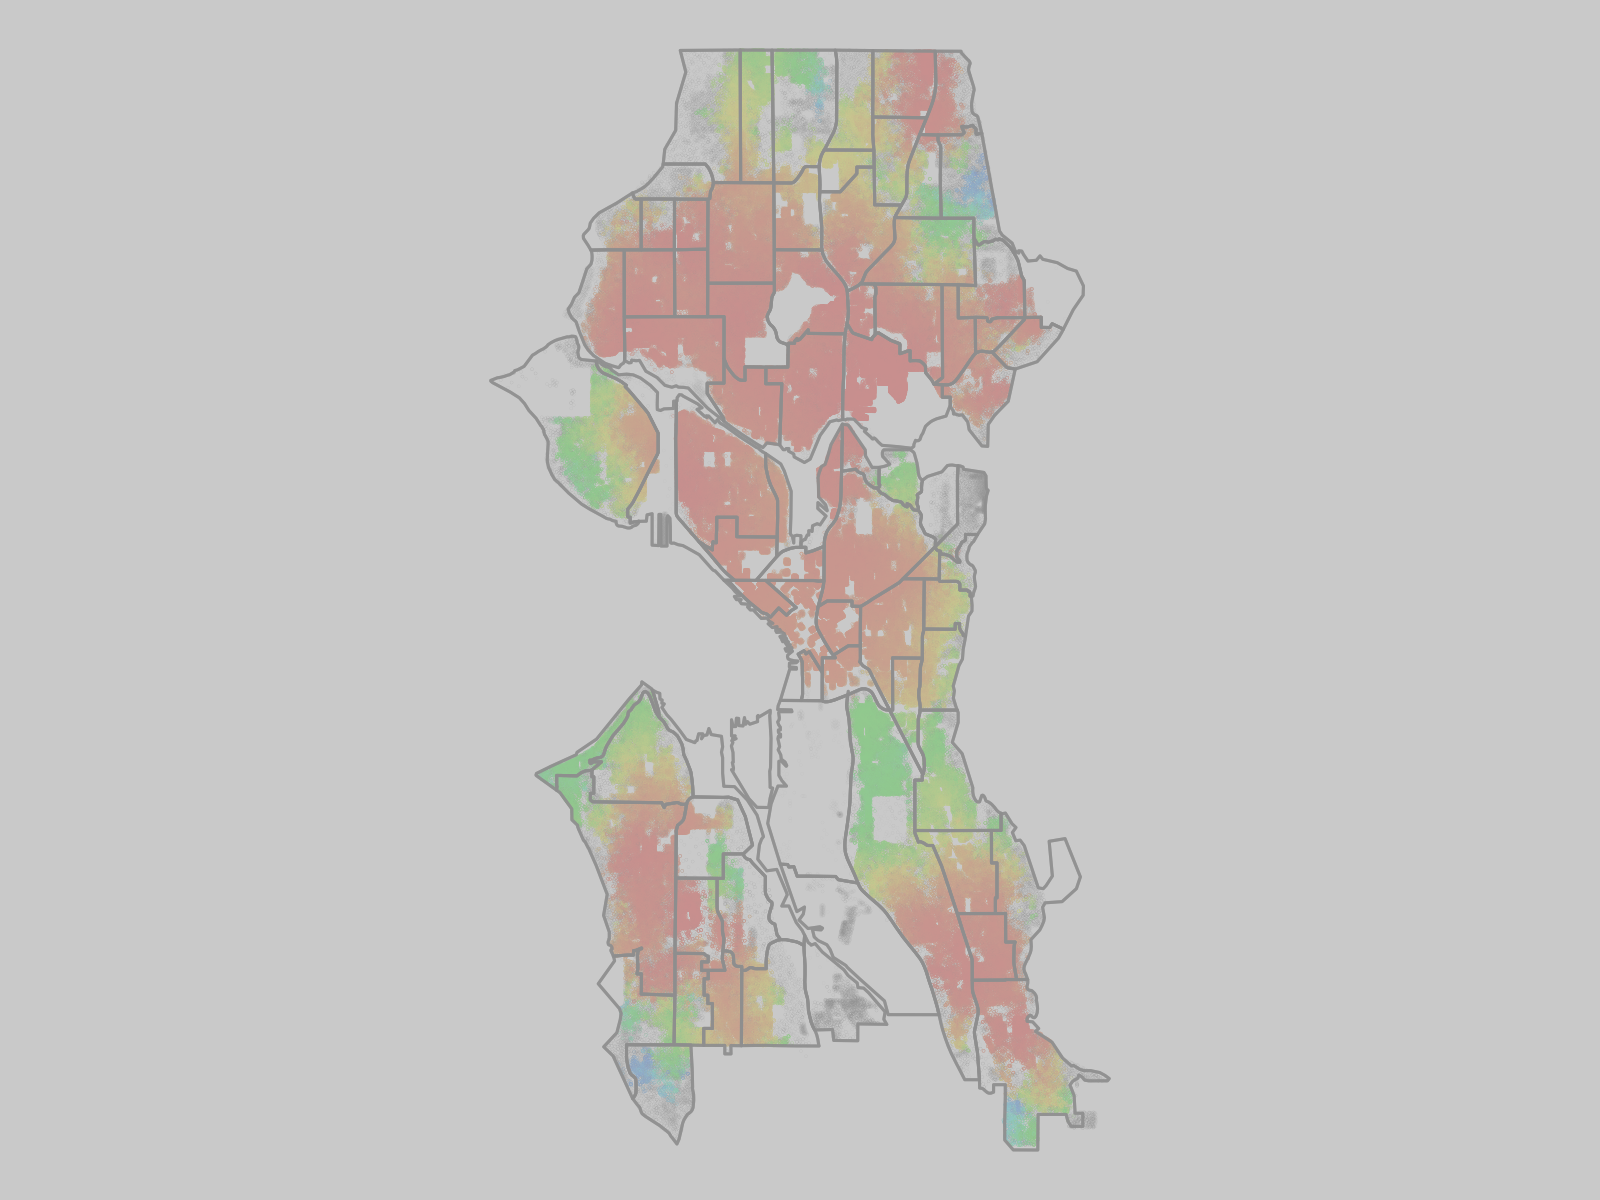
\includegraphics[width=\paperwidth]{graphics/seattle.png}}
\begin{frame}[plain]
  \titlepage
\end{frame}
}

\section[Outline]{}
\begin{frame}[allowframebreaks,plain]{}
\vspace{.25in}
\hspace{.5in}\tableofcontents
\end{frame}




\section{Simple Random Sampling}
\begin{frame}{}
\begin{block}{}
\begin{center}
Simple Random Sampling
\end{center}
\end{block}
\end{frame}

\begin{frame}{Overview}

\begin{block}{Goal}
\begin{itemize}
\item Interest in a function (e.g., mean) from a known population.

\begin{itemize}
\item The number of people who live in Washington.
\item The number of people who own an SUV.
\item The number of people who own an iPhone.
\item The number of people with access to the internet.
\item The average income of an individual who lives in the Seattle.
\item The average age of a person who lives in Minnesota.
\item The percentage of students who passed the state curriculum exams in 4th grade.
\item The proportion of individuals who are registered to vote.
\item The proportion of individuals who are registered to vote who intend to vote.
\item The proportion of individuals who plan to vote Republican.
\item The proportion of individuals who plan to vote Democrat.
\item The proportion of individuals who plan approve of proposition XX.
\end{itemize}

\end{itemize}
\end{block}

\end{frame}

\begin{frame}{Overview}

\begin{block}{Goal}
\begin{itemize}
\item One option, take a census. \only<2>{\textbf{Count Everyone!}}
\end{itemize}
\end{block}

\end{frame}

\begin{frame}{Why sample at all?}

\begin{block}{}
\begin{itemize}
\item Collecting a sample can be cheaper, quicker and even more accurate than
taking a census.
\item The design of the sample is much more important than the size.
\item Important to balance Sampling vs Nonsampling error.
\item Etc.
\end{itemize}
\end{block}
\end{frame}

\begin{frame}{Framework for Probability Sampling}
\begin{block}{}
\begin{center}
Some Examples of Real Sampling Frames!
\end{center}
\end{block}
\end{frame}


\begin{frame}[containsverbatim]{HouseHolds in Irvine, CA}
\begin{center}
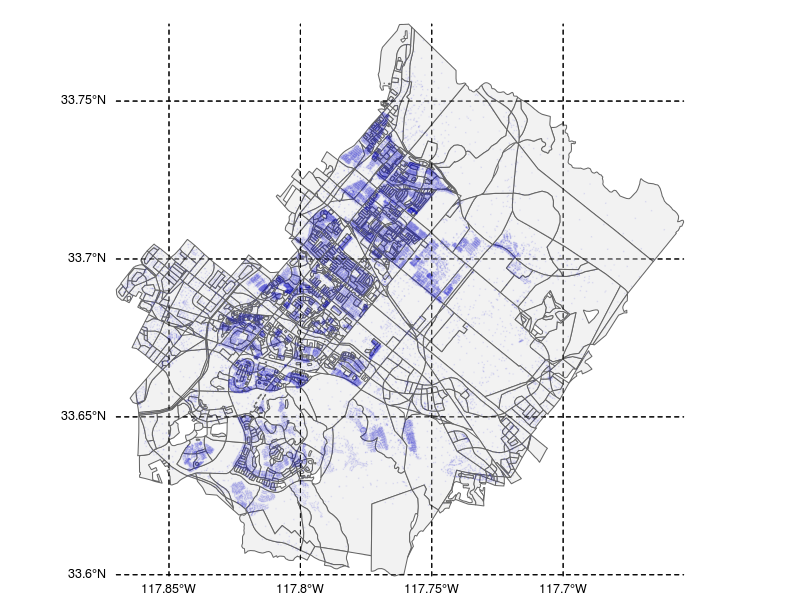
\includegraphics[width=.75\linewidth]{figures/irvineBLK.png}

{\footnotesize Almquist and Butts (2012)}
\end{center}
\end{frame}

\begin{frame}[containsverbatim]{Public Libraries in the US}
\begin{center}
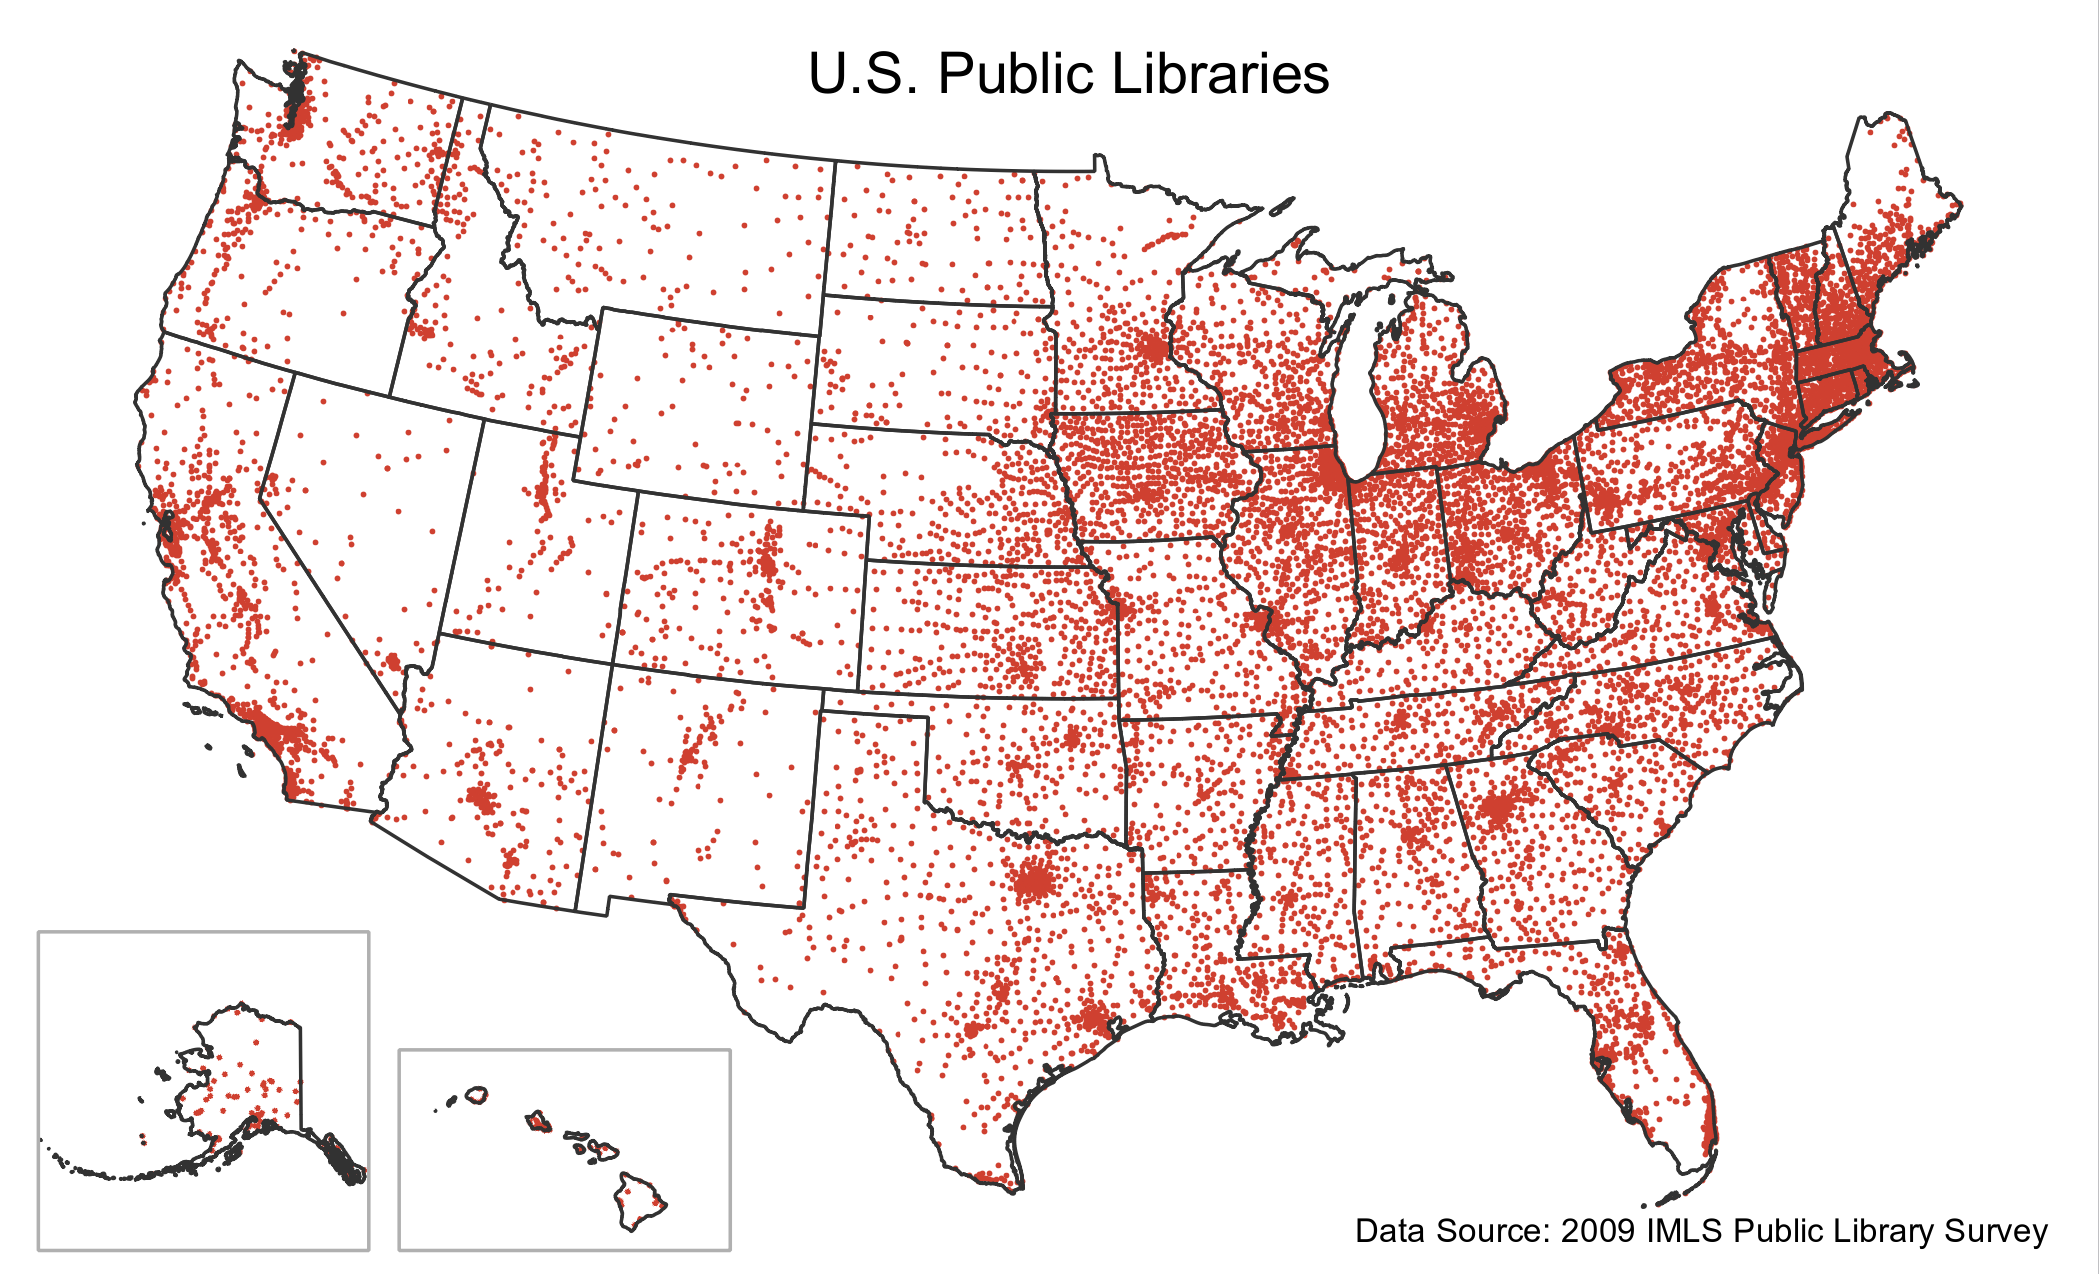
\includegraphics[width=.8\linewidth]{figures/publibs_2009.png}
\end{center}
\end{frame}




\begin{frame}{Overview: Vocabulary}

\begin{block}{Vocabulary}
\begin{itemize}
\item\textbf{Observation unit}
\item \textbf{Target population}
\only<2>{ 
\begin{itemize}
\item {\bf Target population} $=\mathcal{U}=$ population of interest.
\end{itemize}
}
\item \textbf{Sample}
\item \textbf{Sampled population}

\only<3>{ 
\begin{itemize}
\item  {\bf Sampled population} is the collection of all the possible units 
we could see in our sample.
\end{itemize}
}

\item \textbf{Sampling unit}

\only<4>{ 
\begin{itemize}
\item  {\bf Sampling unit} is what we can actually sample. We may be interested 
in individuals but only have a list of households.
\end{itemize}
}

\item \textbf{Sampling frame}

\only<5>{ 
\begin{itemize}
\item  {\bf Sampling frame} is the complete list of sampling units.
\end{itemize}
}

\end{itemize}
\end{block}
\end{frame}

\begin{frame}{Sampling Distribution}
\begin{block}{}
Most results in \underline{sampling} rely on the \underline{sampling distribution} of a statistic, the distribution of different values of the statistic obtained by the process of taking all possible samples from the population. 

\begin{itemize}
\item A sampling distribution is an example of a \emph{discrete probability distribution}.
\end{itemize}
\end{block}
\end{frame}


\begin{frame}{Framework for Probability Sampling}
The finite \textbf{population}, or \textbf{universe}, of $N$ units is denoted by the index set $$\mathcal{U}=\{1,2,3,\dots,N\}$$
\end{frame}

\begin{frame}{Basic Notation}

\begin{itemize}
\item $\{ y_1,y_2,\dots,y_N\}\;\textrm{is a finite population}$ (Notice that this is sometimes referred to as $\mathcal{U}$.
\item It contains $N$ units where $N$ is known.
\item $i$ is the label identifying a unit.
\item The $y_i$'s are the values of the characteristic of interest and are unknown.
\item We may select (how?) $n$ units from the population and use them to
estimate the population mean.
\item $\mathcal{U}$ is a class of 45 students and $y_i$ is the year the mother 
of the $i$th student was born.
\item Let $smp$ be the labels of the $n$ students selected in the sample. Then
the sample mean $= \ybara = \ybarb$  could be a  good guess for the population mean $=\ytot/N$.
\end{itemize}
\end{frame}


\subsection{Simple Random Sampling Definitions}

\begin{frame}{Simple Random Sampling}

\begin{itemize}
\item SRS With Replacement (SRSWR)
\item SRS Without Replacement (SRS)
\end{itemize}

\end{frame}


\subsection{Simple Random Sample without Replacement}
\begin{frame}[containsverbatim]{SRS}
\small

\begin{knitrout}
\definecolor{shadecolor}{rgb}{1, 1, 1}\color{fgcolor}\begin{kframe}
\begin{alltt}
\hlstd{s} \hlkwb{<-} \hlkwd{sample}\hlstd{(}\hlnum{1}\hlopt{:}\hlnum{100}\hlstd{,} \hlnum{30}\hlstd{,} \hlkwc{replace} \hlstd{=} \hlnum{FALSE}\hlstd{)}
\hlstd{s}
\end{alltt}
\begin{verbatim}
 R >   [1]  1 90 27 72 15 38 95 76 29 58 18 67
 R >  [13] 77 37 26 57 89 50 10 82 41 79 44 56
 R >  [25] 75 33 23 16 97 83
\end{verbatim}
\end{kframe}
\end{knitrout}

\end{frame}


\subsection[containsverbatim]{SRS with Replacement}
\begin{frame}[containsverbatim]{SRSWR}
\small
\begin{knitrout}
\definecolor{shadecolor}{rgb}{1, 1, 1}\color{fgcolor}\begin{kframe}
\begin{alltt}
\hlstd{s} \hlkwb{<-} \hlkwd{sample}\hlstd{(}\hlnum{1}\hlopt{:}\hlnum{100}\hlstd{,} \hlnum{30}\hlstd{,} \hlkwc{replace} \hlstd{=} \hlnum{TRUE}\hlstd{)}
\hlstd{s}
\end{alltt}
\begin{verbatim}
 R >   [1] 47 98 46 42 20 94 60 24 93 29 24  6
 R >  [13] 64 36  8 19 59 90 71 52 43 90 59 38
 R >  [25] 97 39 91 62 95 25
\end{verbatim}
\end{kframe}
\end{knitrout}

\end{frame}


\subsection{SRS Weights}
\begin{frame}{SRS Weights}
\only<1>{
\begin{block}{The probability that unit $i$ of the population appears in the sample is}
$$\pi_i = \frac{n}{N}$$
\end{block}
}
\only<2-3>{
\begin{block}{The sampling weight for each unit in the sample is}
$$w_i = \frac{1}{\pi_i} = \frac{N}{n}$$
\end{block}
}
\only<3>{
\begin{itemize}
\item Each unit in the sample can be thought of as representing $\frac{N}{n}$ units in the population.
\begin{itemize}
\item E.g., A sample of 300 from Minnesota, means that an individual from the sample represents $\frac{5,420,380}{300}=18,067.93$ Minnesotans.
\end{itemize}
\end{itemize}
}
\end{frame}

\subsection{Estimation}
\begin{frame}{Estimates and Variance}
\small
\begin{tabular}{lcc}
Population Quantity & Estimator & Standard Error of Estimator\\
\hline
Population total,  $t=\sum_{i=1} y_i$ & $\hat{t} = \sum_{i\in S} w_i y_i = N\bar{y}$&$N\sqrt{\left( 1-\frac{n}{N}\right)\frac{s^2}{n}}$\\
&&\\
Population mean, $\bar{y}_{\mathcal{U}} = \frac{t}{N}$ & $\frac{\hat{t}}{N} \frac{\sum_{i\in S} w_i y_i }{\sum_{i\in S} w_i}=\bar{y}$ & $\sqrt{\left( 1-\frac{n}{N}\right)\frac{s^2}{n}}$\\
&&\\
Population proportion, $p$ & $\hat{p}$ & $\sqrt{\left(1-\frac{n}{N}\right)\frac{\hat{p}(1-\hat{p})}{n-1}}$
\end{tabular}

\begin{itemize}
\item $\bar{y}_{\mathcal{U}} = \sum_{i=1}^N y_i/n$
\item $\bar{y} = \sum_{i \in S} y_i/n$
\item $S^2 = \sum_{i=1}^N (y_i-\bar{y}_{\mathcal{U}})^2/(N-1)$
\item $s^2 = \sum_{i \in S} (y_i-\bar{y})^2/(n-1)$
\item \textbf{Key Properties:} Unbiased or biased and S.E.
\end{itemize}
\end{frame}


\begin{frame}[containsverbatim]{Examples: SRS}
\tiny
\begin{knitrout}
\definecolor{shadecolor}{rgb}{1, 1, 1}\color{fgcolor}\begin{kframe}
\begin{alltt}
\hlstd{readGSS} \hlkwb{<-} \hlkwa{function}\hlstd{(}\hlkwc{address}\hlstd{,} \hlkwc{zipFile}\hlstd{) \{}
    \hlkwd{require}\hlstd{(foreign)}  \hlcom{### for read.dta function}
    \hlstd{fileName} \hlkwb{<-} \hlkwd{paste}\hlstd{(address, zipFile,} \hlkwc{sep} \hlstd{=} \hlstr{""}\hlstd{)}  \hlcom{##full address of zip file}
    \hlstd{zipdir} \hlkwb{<-} \hlkwd{tempfile}\hlstd{()}  \hlcom{### Create temp file}
    \hlkwd{dir.create}\hlstd{(zipdir)}  \hlcom{### Create a folder in the temp file}
    \hlkwd{download.file}\hlstd{(fileName,} \hlkwc{destfile} \hlstd{=} \hlkwd{paste}\hlstd{(zipdir,}
        \hlstd{zipFile,} \hlkwc{sep} \hlstd{=} \hlstr{"/"}\hlstd{))}  \hlcom{## Download the zip file}
    \hlkwd{unzip}\hlstd{(}\hlkwd{paste}\hlstd{(zipdir, zipFile,} \hlkwc{sep} \hlstd{=} \hlstr{"/"}\hlstd{),}
        \hlkwc{exdir} \hlstd{= zipdir)}  \hlcom{### Extract the zip file}
    \hlstd{files} \hlkwb{<-} \hlkwd{list.files}\hlstd{(zipdir)}  \hlcom{## Get the name (assumes it is the second file after the zip)}
    \hlkwd{read.dta}\hlstd{(}\hlkwd{paste}\hlstd{(zipdir, files[}\hlnum{2}\hlstd{],} \hlkwc{sep} \hlstd{=} \hlstr{"/"}\hlstd{))}  \hlcom{### read in the file and output data.frame}
\hlstd{\}}
\hlstd{GSS2012} \hlkwb{<-} \hlkwd{readGSS}\hlstd{(}\hlstr{"https://gss.norc.org/documents/stata/"}\hlstd{,}
    \hlstr{"2012_stata.zip"}\hlstd{)}
\hlstd{lookup} \hlkwb{<-} \hlkwa{function}\hlstd{(}\hlkwc{data}\hlstd{,} \hlkwc{var}\hlstd{) \{}
    \hlstd{out} \hlkwb{<-} \hlkwd{names}\hlstd{(data)[}\hlkwd{grep}\hlstd{(var,} \hlkwd{names}\hlstd{(data))]}
    \hlkwd{print}\hlstd{(}\hlkwd{head}\hlstd{(data[, out]))}
    \hlkwd{invisible}\hlstd{(out)}
\hlstd{\}}
\end{alltt}
\end{kframe}
\end{knitrout}
\end{frame}

\begin{frame}[containsverbatim]{Examples: SRS}
\tiny
\begin{knitrout}
\definecolor{shadecolor}{rgb}{1, 1, 1}\color{fgcolor}\begin{kframe}
\begin{alltt}
\hlstd{vot} \hlkwb{<-} \hlkwd{lookup}\hlstd{(GSS2012,} \hlstr{"vot"}\hlstd{)}
\end{alltt}
\begin{verbatim}
 R >  [1] did not vote ineligible  
 R >  [3] voted        voted       
 R >  [5] voted        voted       
 R >  6 Levels: voted ... No answer
\end{verbatim}
\begin{alltt}
\hlstd{email} \hlkwb{<-} \hlkwd{lookup}\hlstd{(GSS2012,} \hlstr{"email"}\hlstd{)}
\end{alltt}
\begin{verbatim}
 R >    emailhr emailmin
 R >  1       4       NA
 R >  2      NA       NA
 R >  3      NA       NA
 R >  4       2       NA
 R >  5       0       30
 R >  6      NA        5
\end{verbatim}
\end{kframe}
\end{knitrout}
\end{frame}

\begin{frame}[containsverbatim]{Examples: SRS}
\tiny
\begin{knitrout}
\definecolor{shadecolor}{rgb}{1, 1, 1}\color{fgcolor}\begin{kframe}
\begin{alltt}
\hlstd{educ} \hlkwb{<-} \hlkwd{lookup}\hlstd{(GSS2012,} \hlstr{"educ"}\hlstd{)}
\end{alltt}
\begin{verbatim}
 R >    sei10educ spsei10educ pasei10educ
 R >  1      79.4          NA        65.6
 R >  2      72.5          NA          NA
 R >  3      95.6        98.9          NA
 R >  4      93.7        55.4        85.7
 R >  5      54.8          NA        76.9
 R >  6      97.3          NA        81.0
 R >    masei10educ      coneduc educ
 R >  1          NA         <NA>   16
 R >  2        73.3    only some   12
 R >  3        58.8    only some   12
 R >  4          NA    only some   13
 R >  5        37.0 a great deal   16
 R >  6        57.6         <NA>   19
 R >                  inteduc maeduc
 R >  1                  <NA>     16
 R >  2 moderately interested     12
 R >  3 moderately interested     15
 R >  4 not at all interested     16
 R >  5       very interested     12
 R >  6                  <NA>     12
 R >        nateduc   nateducy paeduc sexeduc
 R >  1        <NA> too little     16   favor
 R >  2        <NA> too little     NA    <NA>
 R >  3  too little       <NA>     NA    <NA>
 R >  4        <NA> too little     18   favor
 R >  5        <NA> too little     NA   favor
 R >  6 about right       <NA>     14   favor
 R >    speduc
 R >  1     NA
 R >  2     NA
 R >  3     16
 R >  4     16
 R >  5     NA
 R >  6     NA
\end{verbatim}
\end{kframe}
\end{knitrout}
\end{frame}



\begin{frame}[containsverbatim]{Examples: SRS}
\tiny
\begin{knitrout}
\definecolor{shadecolor}{rgb}{1, 1, 1}\color{fgcolor}\begin{kframe}
\begin{alltt}
\hlstd{vote} \hlkwb{<-} \hlstd{GSS2012[, vot]}
\hlstd{Ivote} \hlkwb{<-} \hlkwd{as.numeric}\hlstd{(vote} \hlopt{==} \hlstr{"voted"}\hlstd{)}
\hlstd{Ivote} \hlkwb{<-} \hlstd{Ivote[}\hlopt{!}\hlkwd{is.na}\hlstd{(Ivote)]}

\hlcom{## Population Total}
\hlstd{N} \hlkwb{<-} \hlkwd{length}\hlstd{(Ivote)}
\hlstd{N}
\end{alltt}
\begin{verbatim}
 R >  [1] 1948
\end{verbatim}
\begin{alltt}
\hlcom{## Population Total Voters}
\hlstd{t} \hlkwb{<-} \hlkwd{sum}\hlstd{(Ivote)}
\hlstd{t}
\end{alltt}
\begin{verbatim}
 R >  [1] 1304
\end{verbatim}
\begin{alltt}
\hlcom{## Population Mean/Proportion}
\hlstd{p} \hlkwb{<-} \hlkwd{mean}\hlstd{(Ivote)}
\hlstd{p}
\end{alltt}
\begin{verbatim}
 R >  [1] 0.6694045
\end{verbatim}
\begin{alltt}
\hlkwd{set.seed}\hlstd{(}\hlnum{18744}\hlstd{)}
\hlstd{s} \hlkwb{<-} \hlkwd{sample}\hlstd{(}\hlnum{1}\hlopt{:}\hlstd{t,} \hlnum{50}\hlstd{,} \hlkwc{replace} \hlstd{=} \hlnum{FALSE}\hlstd{)}

\hlstd{vote_sample} \hlkwb{<-} \hlstd{Ivote[s]}
\hlstd{phat} \hlkwb{<-} \hlkwd{mean}\hlstd{(vote_sample)}
\hlstd{phat}
\end{alltt}
\begin{verbatim}
 R >  [1] 0.74
\end{verbatim}
\end{kframe}
\end{knitrout}
\end{frame}

\begin{frame}[containsverbatim]{Examples: SRS}
\tiny
\begin{knitrout}
\definecolor{shadecolor}{rgb}{1, 1, 1}\color{fgcolor}\begin{kframe}
\begin{alltt}
\hlstd{sephat} \hlkwb{<-} \hlkwd{sqrt}\hlstd{((}\hlnum{1} \hlopt{-} \hlnum{50}\hlopt{/}\hlstd{N)} \hlopt{*} \hlstd{(phat} \hlopt{*} \hlstd{(}\hlnum{1} \hlopt{-}
    \hlstd{phat)}\hlopt{/}\hlstd{(}\hlnum{50} \hlopt{-} \hlnum{1}\hlstd{)))}
\hlstd{sephat}
\end{alltt}
\begin{verbatim}
 R >  [1] 0.06185262
\end{verbatim}
\begin{alltt}
\hlstd{t_hat} \hlkwb{<-} \hlstd{N} \hlopt{*} \hlstd{phat}
\hlstd{t_hat}
\end{alltt}
\begin{verbatim}
 R >  [1] 1441.52
\end{verbatim}
\begin{alltt}
\hlstd{se_t_hat} \hlkwb{<-} \hlstd{N} \hlopt{*} \hlstd{sephat}
\hlstd{se_t_hat}
\end{alltt}
\begin{verbatim}
 R >  [1] 120.4889
\end{verbatim}
\end{kframe}
\end{knitrout}
\end{frame}





\subsection{Confidence Interval}
\begin{frame}{Confidence Interval}

\only<1>{
\begin{block}{}
\begin{center}
estimate $\pm$ $z_{\alpha/2}$ SE(estimate) 
\end{center}
\end{block}
}
\only<2>{
\begin{block}{$100(1-\alpha)\%$ CI for the Population Mean}
$$\left[ \bar{y} - z_{\alpha/2}\sqrt{1-\frac{n}{N}} \frac{S}{\sqrt{n}}\;,\; \bar{y} + z_{\alpha/2}\sqrt{1-\frac{n}{N}} \frac{S}{\sqrt{n}}\right]$$
\end{block}
}
\only<3>{
\begin{block}{$100(1-\alpha)\%$ CI for the Population Mean (t-distribution)}
$$\left[ \bar{y} - t_{\alpha/2,n-1}\sqrt{1-\frac{n}{N}} \frac{S}{\sqrt{n}}\;,\; \bar{y} + t_{\alpha/2,n-1}\sqrt{1-\frac{n}{N}} \frac{S}{\sqrt{n}}\right]$$
\end{block}

\begin{itemize}
\item For large samples, $t_{\alpha/2,n-1} \approx z_{\alpha/2}$.
\item In smaller samples, using $t_{\alpha/2,n-1}$ instead of $z_{\alpha/2}$ produces wider CI.
\item In practice (and most software) one uses t approximation (b/c it is more conservative).
\end{itemize}
}

\end{frame}


\begin{frame}[containsverbatim]{Examples: total and p CI for SRS}
\small
\begin{knitrout}
\definecolor{shadecolor}{rgb}{1, 1, 1}\color{fgcolor}\begin{kframe}
\begin{alltt}
\hlcom{## Total}
\hlstd{t_hat} \hlopt{+} \hlkwd{qt}\hlstd{(}\hlnum{0.025}\hlstd{,} \hlnum{50} \hlopt{-} \hlnum{1}\hlstd{)} \hlopt{*} \hlstd{se_t_hat}
\end{alltt}
\begin{verbatim}
 R >  [1] 1199.388
\end{verbatim}
\begin{alltt}
\hlstd{t_hat} \hlopt{+} \hlkwd{qt}\hlstd{(}\hlnum{0.025}\hlstd{,} \hlnum{50} \hlopt{-} \hlnum{1}\hlstd{,} \hlkwc{lower.tail} \hlstd{=} \hlnum{FALSE}\hlstd{)} \hlopt{*}
    \hlstd{se_t_hat}
\end{alltt}
\begin{verbatim}
 R >  [1] 1683.652
\end{verbatim}
\begin{alltt}
\hlcom{## Proportion}
\hlstd{phat} \hlopt{+} \hlkwd{qt}\hlstd{(}\hlnum{0.025}\hlstd{,} \hlnum{50} \hlopt{-} \hlnum{1}\hlstd{)} \hlopt{*} \hlstd{sephat}
\end{alltt}
\begin{verbatim}
 R >  [1] 0.6157025
\end{verbatim}
\begin{alltt}
\hlstd{phat} \hlopt{+} \hlkwd{qt}\hlstd{(}\hlnum{0.025}\hlstd{,} \hlnum{50} \hlopt{-} \hlnum{1}\hlstd{,} \hlkwc{lower.tail} \hlstd{=} \hlnum{FALSE}\hlstd{)} \hlopt{*}
    \hlstd{sephat}
\end{alltt}
\begin{verbatim}
 R >  [1] 0.8642975
\end{verbatim}
\end{kframe}
\end{knitrout}
\end{frame}

\subsection{Sample Size Estimation}

\begin{frame}{}
\begin{block}{}
Sample Size Estimation
\end{block}
\end{frame}

\begin{frame}{Sample size estimation}

\begin{block}{}
\textbf{Sample size is never large enough}. As $n$ increases, we estimate more interactions,
which typically are smaller and have relatively larger standard errors than main
effects.\\ - Andrew Gelman (Professor in Statistics at Columbia University)
\end{block}

\end{frame}

\begin{frame}{Sample size estimation}

\begin{block}{}
Two Core Objectives
\end{block}

\begin{itemize}
\item Measure with a precision:
\begin{itemize}
\item Precision analysis
\end{itemize}
\item Assure that the difference is correctly detected
\begin{itemize}
\item Power analysis
\end{itemize}
\end{itemize}

\end{frame}

\begin{frame}{Sample size estimation}

\begin{block}{Precision}
Whenever we propose to estimate 
population parameters, such as, 
population mean, proportion, or total, 
we need to estimate with a \textbf{specified 
level of precision}
\end{block}

\begin{block}{}
We like to specify a sample size that 
is sufficiently large to ensure a high 
probability that errors of estimation 
can be limited within desired limits
\end{block}

\end{frame}

\begin{frame}{Sample size estimation}

\begin{block}{Power}
The power of a test is the probability of rejecting the null hypothesis 
if it is incorrect.
\end{block}
\end{frame}

\begin{frame}{SRS and Precision}

\begin{block}{Lohr Algorithm 2.6}
\begin{enumerate}
\item Ask: ``What is expected of the sample, and how much precision do I need?"
\item Find an equation relating the sample size $n$ and your expectations of the sample.
\item Estimate any unknown quantities and solve for $n$. 
\begin{itemize}
\item Use known data
\item Simulate
\item Use prior knowledge to build bounds
\end{itemize}
\item[*]\textbf{Lessons}: You will likely realize that the sample you should get is more expensive than you can possible do; carefully go through your assumptions and ask what outcomes, what level of precision, etc you are willing to give up\dots
\end{enumerate}
\end{block}

\end{frame}

\begin{frame}{SRS and Precision}
\begin{block}{Specify the Tolerable Error}
$$\Pr(|\bar{y}-\bar{Y}_{\mathcal{U}}| \leq e) = 1-\alpha$$
\end{block}

\begin{block}{Goal}
\begin{itemize}
\item The investigator must decide on reasonable values for $\alpha$ and $e$

\begin{itemize}
\item $e$ is called the \textbf{margin of error} in many surveys
\item Lohr notes that $e=0.03$ and $\alpha=0.05$ in many surveys
\end{itemize}

\end{itemize}
\end{block}

\end{frame}


\begin{frame}{SRS and Precision}

\begin{block}{Relative precision}
Can be achieved by controlling Coefficient of Variation (CV) rather than the absolute error; in this case, if $\bar{Y}_{\mathcal{U}} \neq 0$ the precision may be expressed as 
$$\Pr\left(\left| \frac{\bar{y}-\bar{Y}_{\mathcal{U}}}{\bar{Y}_{\mathcal{U}}}\right| \leq r \right) = 1-\alpha$$
\end{block}

\end{frame}


\begin{frame}{SRS and Precision}

\begin{block}{Find an equation}
The simplest equation relating the precision and sample size comes from the formal for confidence intervals. To obtain absolute precision $e$, find a value of $n$ that satisfies
$$e=z_{\alpha/2}\sqrt{(1-\frac{n}{N})}\frac{S}{\sqrt{n}}$$
\end{block}
\end{frame}


\begin{frame}{SRS and Precision}

\begin{block}{SRSWR (Easy case)}

$$n_0 = \left(\frac{z_{\alpha/2}S}{e}\right)^2$$

\end{block}

\begin{itemize}
\item Obvious if $n_0>N$ we just a census with $n=N$
\end{itemize}

\end{frame}


\begin{frame}{SRS and Precision}

\begin{block}{SRS}
$$n = \frac{n_0}{1+\frac{n_0}{N}} = \frac{z_{\alpha/2}^2S^2}{e^2+\frac{z_{\alpha/2}^2S^2}{N}}$$
\end{block}

\end{frame}

\begin{frame}{Example 2.12}

\begin{block}{}
\begin{itemize}
\item Many public opinion polls specify using a sample size of about 1,100.
\item That number comes from rounding the value of $n_0$ (from SRSWR) and noting that the population size is so large that the fpc can be ignored (i.e., 1100/300,000,000=0.000003667). 
\item For large populations, it is the size of the sample, not the proportion of the population that is sampled, that determines the precision.
\end{itemize}
\end{block}

\end{frame}

\begin{frame}{Example 2.12}

\begin{block}{}
\begin{itemize}
\item When interested in a proportion, we can use 1/4 as an upper bound for $S^2$. For other quantities, $S^2$ must be estimated or guessed at. Some methods for estimating $S^2$ include:

\begin{enumerate}
\item Use sample quantities obtained when pretesting your survey (e.g., pilot study)
\item Use previous studios or data available in the literature.
\item Make an a guess! (There a better and worse ways to do such a thing)
\end{enumerate}

\end{itemize}
\end{block}

\end{frame}


\subsection{Systematic Sampling}

\begin{frame}{}
\begin{block}{}
Systematic Sampling
\end{block}
\end{frame}

\begin{frame}{Systematic Sampling}
\begin{block}{}
\begin{itemize}
\item \textbf{Systematic sampling} is used as a proxy for SRS when 
\begin{itemize}
\item No list of the population exists
\item Or when the list is in roughly random order
\end{itemize}
\end{itemize}
\end{block}
\end{frame}

\begin{frame}{Systematic Sampling}
\begin{block}{}
To obtain a systematic sample, choose a sample size $n$. If $N/n$ is an integer, let $k=N/n$; otherwise, let $k$ be the next integer after $N/n$. Then find a random integer $R$ between 1 and $k$, which determines the sample to be units numbered $R$, $R+k$, $R+2k$, \dots.
\end{block}

\begin{block}{}
For example, to select a systematic sample of 45 students from the list of 45,000 students at a university, the sampling interval $k$ is 1000. Suppose the random integer we choose is 597. Then the students numbered 597, 1597, 2597, \dots, 44,957 would be in the sample.

\begin{itemize}
\item If the list of students is ordered by randomly generated student identification numbers, we shall probably obtain a sample that will behave much like an SRS.
\end{itemize}

\end{block}

\end{frame}

\begin{frame}{Systematic Sampling}
\begin{block}{Issues}
\begin{itemize}
\item If the population is in some periodic or cyclical order.
\begin{itemize}
\item E.g., If male and female names alternate in the list
\end{itemize}
\item If populations are listed in increasing or decreasing order
\item Requires a sampling frame and defining the target population
\end{itemize}
\end{block}
\end{frame}







\subsection{Design-based and Model-based Framework}
\begin{frame}{}
\begin{block}{}
\begin{center}
Design-based and Model-based Frameworks
\end{center}
\end{block}
\end{frame}


\begin{frame}{Overview}

\begin{itemize}
\item \textbf{Design-based} inference: population values are fixed, inference is based on probability distribution of sample selection. Obviously this assumes that we have a probability sample (or ``quasi-randomization", where we pretend that we have one)
\item \textbf{Model-based} inference: survey variables are assumed to come from a statistical model: probability sampling is not the basis for inference, but useful for making the sample selection \textbf{ignorable}. (see e.g. Gelman et al., 2003)
\end{itemize}

\end{frame}

\subsection{Design-Based Approach}
\begin{frame}{}
\begin{block}{}
\begin{center}
Design-Based Approach
\end{center}
\end{block}
\end{frame}

\begin{frame}{Design-Based Approach}
\begin{block}{Also known as Randomization Theory}
\begin{itemize}
\item No distributional assumptions are made about the $y_i$'s to ascertain that $\bar{y}$ is unbiased for estimating $\bar{y}_{\mathcal{U}}$
\item We treat the $y_i$'s as fixed but unknown numbers
\item The RV used in randomization theory inference indicate which population units are in the sample
\end{itemize}
\end{block}
\end{frame}

\begin{frame}{Design-Based Approach}
$$Z_i =     \left\{ \begin{array}{cl}
1 & \textrm{ if unit $i$ is in the sample}\\
0 & \textrm{ otherwise}
   \end{array}
   \right.$$
\end{frame}


\begin{frame}{Design-Based Approach}
\only<1>{
\begin{block}{The Mean}
$$ \bar{y} = \sum_{i \in S} \frac{y_i}{n} = \sum_{i=1}^N Z_i \frac{y_i}{n}$$
\end{block}
}
\only<2>{
\begin{block}{RV}
The $Z_i$'s are the only random variable because, according to randomization theory, the $y_i$'s are fixed quantities.
\end{block}
}
\only<3>{
\begin{block}{RV}
When we choose an SRS of $n$ units out of the $N$ units in the population, $\{Z_1,\dots,Z_N\}$ are identically distributed Bernoulli random variables with
$$\pi_i = \Pr(Z_i=1)=\Pr(\textrm{ select unit $i$ in the sample}) =\frac{n}{N}$$
and
$$P(Z_i=0)=1-\pi_i = 1-\frac{n}{N}$$
\end{block}
}
\only<4>{
\begin{block}{Proof that $\bar{y}$ is unbiased}
$$P(Z_i=1) = \frac{\textrm{\# of samples including unit $i$}}{\textrm{\# number of possible samples}} = \frac{{N-1 \choose n-1}}{{N \choose n}} = \frac{n}{N}$$
\end{block}
}
\only<5>{
\begin{block}{Proof that $\bar{y}$ is unbiased}
Notice that $E[Z_i]=E[Z_i^2]=\frac{n}{N}$.
\end{block}
}
\only<6>{
\begin{block}{Proof that $\bar{y}$ is unbiased}
$$E[\bar{y}] = E\left[ \sum_{i=1}^N Z_i \frac{y_i}{n} \right] = \dots = \bar{y}_{\mathcal{U}}$$
\end{block}
}
\only<7>{
\begin{block}{Variance of $\bar{y}$}
$$V(Z_i) = E[Z_i^2]-(E[Z_i])^2 = \dots = \frac{n}{N}\left( 1-\frac{n}{N}\right)$$
for $i\neq j$
\begin{align*}
 E[Z_iZ_j] &= \Pr(Z_i = 1 \textrm{ and } Z_j = 1) \\
 &= \Pr(Z_j=1 | Z_i =1)P(Z_i=1)\\
 & = \left( \frac{n-1}{N-1}\right)\left( \frac{n}{N}\right)
 \end{align*}
\end{block}
}
\only<8>{
\begin{block}{Variance of $\bar{y}$}
Note that b/c the population is finite, the $Z_i$'s are not quite independent, i.e., if we know that unit $I$ is in the sample, we do have a small amount of information about whether unit $j$ is in the sample, reflected in the conditional probability $\Pr(Z_j=1 | Z_i=1)$. 
\end{block}
}
\only<9>{
\begin{block}{Variance of $\bar{y}$}
\begin{align*}
i\neq j&\\
Cov(Z_i,Z_j) &= E[Z_iZ_j] - E[Z_i]E[Z_j]\\
&= \frac{n-1}{N-1} \frac{n}{N} - \left( \frac{n}{N}\right)^2\\
&= - \frac{1}{N-1} \left( 1-\frac{n}{N}\right) \left( \frac{n}{N}\right)
\end{align*}
\end{block}
}
\only<10>{
\begin{block}{Variance of $\bar{y}$}
The negative covariance of $Z_i$ and $Z_j$ is the source of the fpc!
\end{block}
}
\only<11>{
\begin{block}{Variance of $\bar{y}$}
$$V(\bar{y}) = (1-\frac{n}{N}) \frac{S^2}{n}$$
\end{block}
}
\only<12>{
\begin{block}{Variance of $\bar{y}$}
To show that $V(\bar{y}) = (1-\frac{n}{N}) \frac{S^2}{n}$ is unbiased estimator of the variance we need to show that $E[s^2] =S^2$. Remember, $S^2= \frac{1}{N-1} \sum_{i=1}^N (y_i-\bar{y}_{\mathcal{U}})^2$.
\end{block}
}
\only<13>{
\begin{block}{Variance of $\bar{y}$}
\begin{align*}
E\left[ \sum_{i\in S} (y_i-\bar{y}_{\mathcal{U}})^2\right] = \dots = (n-1)S^2
\end{align*}
\end{block}
}
\only<14>{
\begin{block}{Variance of $\bar{y}$}
\begin{align*}
E\left[ \frac{1}{n-1} \sum_{i \in S} (y_i-\bar{y})\right] = E[s^2] = S^2.
\end{align*}
\end{block}
}
\end{frame}


\subsection{Model-based Approach}

\begin{frame}{}
\begin{block}{}
\begin{center}
Model Based Approach
\end{center}
\end{block}
\end{frame}


\begin{frame}{Model Based Approach}

\begin{itemize}
\item In the design-based approach the $y_i$'s could be anything! Only the inclusion probabilities (the $Z_i$'s were random!)
\item You may be more familiar with the $y_i$'s being random variables?
\item For example, say $Y_1,Y_2,\dots, Y_n$ were independent identically distributed from a $N(\mu,\sigma)$.
\item Where estimators/etc were derived from the independence and distributional assumptions.
\end{itemize}

\end{frame}

\begin{frame}{Model Based Approach}

\begin{block}{}
We can extend this approach to sampling by thinking of random variables $Y_1,Y_2,\dots, Y_N$ generated from some model. 

\begin{itemize}
\item The actual values for the finite population, $y_1,y_2,\dots,y_N$, are one realization of the random variables.
\end{itemize}

\end{block}

\end{frame}

\begin{frame}{Model Based Approach}

\begin{block}{}

\begin{itemize}
\item The joint probability distribution of $Y_1, Y_2,\dots,Y_N$ supplies the link between units in the sample and units not in the sample in this \textbf{model-based} approach.
\item A link that is missing in the randomization approach.
\item Here, we sample $\{y_i,\; i\in S\}$ and use these data to predict the unobserved values $\{y_i,\; i \notin S\}$.
\item Thus, the problems in finite population sampling may be thought of as prediction problems.
\end{itemize}
\end{block}

\end{frame}

\begin{frame}{Model Based Approach}

\begin{block}{In SRS, a simple model is}
$Y_1,\dots,Y_N$ independent with $E_M[Y_j]=\mu$ and $V_M=\sigma^2$. 
\begin{itemize}
\item $M$ denotes that the expectation is taken over the model.
\item $\mu$ and $\sigma^2$ represent unknown infinite population parameters, not the finite population quantities.
\item This model makes assumptions about the observations not in the sample; namely, that they have the same mean and variance as observations that are in the sample. 
\item We take a sample $S$ and observe the values $y_i$ for $i\in S$. That is, we realizations of the RV $Y_i$ for $i\in S$.
\item The other observations in the population $\{y_i,\; i\notin S\}$ are also realizations of random variables, but we do not see those. 
\end{itemize}
\end{block}

\end{frame}

\begin{frame}{Model Based Approach}

\only<1>{
\begin{block}{total}
$$t= \sum_{i=1}^N y_i = \sum_{i \in S} y_i + \sum_{i\notin S} y_i$$
and is one possible value that can be taken on by the random variable
$$T=\sum_{i=1}^N Y_i = \sum_{i \in S} Y_i + \sum_{i\notin S} Y_i$$
\end{block}
}
\only<2>{
\begin{block}{total}
\begin{itemize}
\item We know the values $\{y_i,\; i\in S\}$.
\item To estimate $t$ for our sample, we need to predict values for the $y_i$'s not in the sample. 
\item This is where our model of the common mean $\mu$ comes in.
\item The least squares estimator of $\mu$ from the sample is $\bar{Y}_S = \sum_{i \in S} Y_i/n$.
\item That is the best linear unbiased predictor (under the model) of each unobserved RV.
\end{itemize}
\end{block}
}
\only<3>{
\begin{block}{total}
$$\hat{T} = \sum_{i\in S} Y_i + \sum_{i \notin S} \hat{Y}_i = \sum_{i\in S} Y_i  + \frac{N-n}{n} \sum_{i \in S} Y_i = \frac{N}{n} \sum_{i\in S} Y_i$$
\end{block}
}
\only<4>{
\begin{block}{total}
\begin{itemize}
\item The estimator $\hat{T}$ is model-unbiased: if the model is correct, then the average of $\hat{T}-T$ over repeated realizations of the population is 
$$E_M[\hat{T}-T] = \frac{N}{n} \sum_{i\in S} E_M[Y_i] - \sum_{i=1}^N E_M[Y_i] =0.$$
\end{itemize}
\end{block}
}
\end{frame}

\begin{frame}{Model Based Approach}
\begin{block}{}
Notice the difference between finding expectations under the model-based approach and under the design-based approach. In the model-based approach, the $Y_i$'s are the random variables, and the sample has no information for calculating expected values, so we can take the $\sum_{i \in S}$ outside the expected value. In the design-based approach, the random variables are contained in the sample $S$.
\end{block}
\end{frame}

\begin{frame}{Model Based Approach}
\begin{block}{Mean Square Error}
$$(\hat{t} -t)^2 = \left[ \frac{N}{n} \sum_{i \in S} y_i - \sum_{i=1}^N y_i \right]^2.$$
\end{block}
\end{frame}

\begin{frame}{Model Based Approach}
\begin{block}{Mean Square Error}
$$E_M\left[ (\hat{T}-T)^2)\right] = \dots = N^2(1-\frac{n}{N}) \frac{\sigma^2}{n}.$$
\end{block}
\begin{itemize}
\item In practice, if the model assumed were adopted, you would estimate $\sigma^2$ by the sample variance $s^2$.
\end{itemize}
\end{frame}


\begin{frame}{Model Based Approach v Design-Based Approach}
\begin{itemize}
\item Thus the design-based approach and the model-based approach (in this case) lead to the same estimator of the population total and the same variance estimator. However, this is not guaranteed! If one selects a different model, the estimator could be different.
\item The CI is also the same under this model!
\end{itemize}
\end{frame}


\section{Stratified Random Sampling}

\begin{frame}{}
\begin{block}{}
\begin{center}
Stratified Random Sampling
\end{center}
\end{block}
\end{frame}

\begin{frame}{Stratified Sampling}
\only<1>{
\begin{block}{Why Stratified Sampling}
 Populations can be extremely heterogenous and it is easy for a single SRS to miss some of this heterogeneity. 
\end{block}
Examples:
 \begin{itemize}
 \item We know that on average men earn more than women.
 \item We know that NYC residents typically pay more for housing than residents of Des Moines.
 \item That rural residents shop for groceries less often than urban residents.
 \item That internet usage varies by age.
 \item That cell only households are more likely to be younger.
 \item That income varies by state (as does COL).
 \end{itemize}

}
\only<2>{
\begin{block}{Goal}
\begin{itemize}
\item To maximize the representative nature of our sample using known information.
\end{itemize}
\end{block}
}
\end{frame}




\begin{frame}{Why we use Stratified  Sampling}

\only<1-3>{
\begin{block}{We want to be protected from the possibility of obtaining a really bad sample.}
\begin{itemize}
\item When taking an SRS of size 100 from a population of 1000 male and 1000 female students
\begin{itemize}
\item Obtaining a sample with no or very few males is theoretically possible
\item<2> \textcolor{red}{This is bad!}
\end{itemize}
\item<3> A solution is to take a SRS of 50 for each gender category.
\end{itemize}
\end{block}
}
\only<4>{
\begin{block}{We may want data of known precision for subgroups of the population.}
\begin{itemize}
\item These subgroups can easily be strata (with careful definitions).
\item Notice that this procedure can result in over sampling one group, e.g.,
\begin{itemize}
\item Two researchers interested in sampling graduates of electrical and mechanical engineering programs at public universities in SoCal stratified their sample by gender.
\item B/c there are many more males in engineering, taking an equal sample in each strata will result in oversampling the female engineers (this might also be done for precision)  
\end{itemize}
\end{itemize}
\end{block}
}
\only<5>{
\begin{block}{A stratified sample may be more convenient to administer and may result in a lower cost for the survey.}
\begin{itemize}
\item  For example: Sampling frames may be constructed differently in different strata, or different sampling designs or field procedures may be used.
\item E.g., A combination of internet based survey instruments, mail and telephone could be used (note this is not without controversy though\dots).
\end{itemize}
\end{block}
}
\only<6>{
\begin{block}{Stratified sampling often gives more precise (having lower variance) estimates for population means and totals.}
\begin{itemize}
\item Examples:
\begin{itemize}
\item Persons of different ages tend to have different blood pressures.
\item If studying the concentration of plants in an area, one would stratify by type of terrain.
\end{itemize}
\item Stratification works for lowering the variance b/c the variance within each stratum is often lower than the variance in the whole population. Prior knowledge can be used to save money in the sampling procedure.
\end{itemize}

\end{block}
}
\end{frame}

\subsection{Theory of Stratified Sampling}
\begin{frame}{Theory of Stratified Sampling}
\textbf{stratified random sampling} population quantities:

\begin{itemize}
\item $y_{hj}=$ value of the $j$th unit in the stratum $h$
\item $t_h=\sum_{j=1}^{N_h} y_{hj}=$ population total in stratum $h$
\item $t=\sum_{h=1}^H t_h =$ population total
\item $\bar{y}_{hU} = \frac{\sum_{j=1}^{N_h} y_{hj}}{N_h} =$ population mean in stratum $h$
\item $\bar{y}_U = \frac{t}{N} = \frac{\sum_{h=1}^H \sum_{j=1}^{N_h} y_{hj}}{N}$ overall population mean
\item $S_h^2 = \sum_{j=1}^{N_h} \frac{(y_{hj}-\bar{y}_{hU})^2}{N_h-1}=$ population variance in stratum $h$
\end{itemize}
\end{frame}

\begin{frame}{Theory of Stratified Sampling}
Corresponding quantities for the sample, using SRS estimators within each stratum are:

\begin{itemize}
\item $\bar{y}_h = \frac{1}{n_h} \sum_{j \in S_h} y_{hj}$
\item $\hat{t}_h = \frac{N_h}{n_h} \sum_{j\in S_h} y_{hj} = N_h \bar{y}_{h}$
\item $s_h^2 = \sum_{j\in S_h} \frac{(y_{hj}-\bar{y}_h)^2}{n_h-1}$ 
\end{itemize}

\end{frame}

\begin{frame}{Theory of Stratified Sampling}
Suppose we only sampled the $h$th stratum. In effect, we have a population of $N_h$ units and take an SRS of $n_h$ units. 

\begin{itemize}
\item We could estimate $\bar{y}_{hU}$ by $\bar{y}_{h}$.
\item $t_h$ by $\hat{t}_h=N_h \bar{y}_h$. 
\item The population total is $t=\sum_{h=1}^H t_h$, see we estimate $t$ by
$$ \hat{t}_{str} = \sum_{h=1}^H \hat{t}_h = \sum_{h=1}^H N_h \bar{y}_h$$
\item We can estimate $\bar{y}_U$ with:
$$\bar{y}_{str} = \frac{\hat{t}_{str}}{N} =\sum_{h=1}^H \frac{N_h}{N} \bar{y}_h$$
\end{itemize}

\end{frame}

\subsection{Example: Homework Hours}
\begin{frame}{}
\begin{block}{}
Example: Homework Hours
\end{block}
\end{frame}

\begin{frame}{Example: Homework Hours}
\begin{block}{National Education Longitudinal Study of 1988}
\url{http://nces.ed.gov/surveys/nels88/pdf/QuickGuide.PDF}
\end{block}
\end{frame}

\begin{frame}[containsverbatim]{Example: Homework Hours}
\tiny
\begin{knitrout}
\definecolor{shadecolor}{rgb}{1, 1, 1}\color{fgcolor}\begin{kframe}
\begin{alltt}
\hlcom{## NELS-88 homework is in hours}
\hlkwd{library}\hlstd{(foreign)}
\hlstd{imm10} \hlkwb{<-} \hlkwd{read.dta}\hlstd{(}\hlkwc{file} \hlstd{=} \hlstr{"https://stats.oarc.ucla.edu/stat/stata/examples/mlm_imm/imm10.dta"}\hlstd{)}
\hlkwd{head}\hlstd{(imm10)}
\end{alltt}
\begin{verbatim}
 R >    schid stuid   ses    meanses homework
 R >  1  7472     3 -0.13 -0.4826087        1
 R >  2  7472     8 -0.39 -0.4826087        0
 R >  3  7472    13 -0.80 -0.4826087        0
 R >  4  7472    17 -0.72 -0.4826087        1
 R >  5  7472    27 -0.74 -0.4826087        2
 R >  6  7472    28 -0.58 -0.4826087        1
 R >    white parented public ratio percmin
 R >  1     1        2      1    19       0
 R >  2     1        2      1    19       0
 R >  3     1        2      1    19       0
 R >  4     1        2      1    19       0
 R >  5     1        2      1    19       0
 R >  6     1        2      1    19       0
 R >    math sex race sctype cstr scsize
 R >  1   48   2    4      1    2      3
 R >  2   48   1    4      1    2      3
 R >  3   53   1    4      1    2      3
 R >  4   42   1    4      1    2      3
 R >  5   43   2    4      1    2      3
 R >  6   57   2    4      1    2      3
 R >    urban region schnum
 R >  1     2      2      1
 R >  2     2      2      1
 R >  3     2      2      1
 R >  4     2      2      1
 R >  5     2      2      1
 R >  6     2      2      1
\end{verbatim}
\end{kframe}
\end{knitrout}
\end{frame}


\begin{frame}[containsverbatim]{Example: Homework Hours}
\small
\begin{knitrout}
\definecolor{shadecolor}{rgb}{1, 1, 1}\color{fgcolor}\begin{kframe}
\begin{alltt}
\hlcom{#### Say we are interested in hour}
\hlcom{#### stratified on public/private}
\hlstd{homework.public} \hlkwb{<-} \hlstd{imm10}\hlopt{$}\hlstd{homework[imm10}\hlopt{$}\hlstd{public} \hlopt{==}
    \hlnum{1}\hlstd{]}
\hlstd{homework.private} \hlkwb{<-} \hlstd{imm10}\hlopt{$}\hlstd{homework[imm10}\hlopt{$}\hlstd{public} \hlopt{==}
    \hlnum{0}\hlstd{]}

\hlstd{N} \hlkwb{<-} \hlkwd{length}\hlstd{(imm10}\hlopt{$}\hlstd{homework)}
\hlstd{N1} \hlkwb{<-} \hlkwd{length}\hlstd{(homework.public)}
\hlstd{N2} \hlkwb{<-} \hlkwd{length}\hlstd{(homework.private)}

\hlstd{n1} \hlkwb{<-} \hlkwd{ceiling}\hlstd{(}\hlnum{0.1} \hlopt{*} \hlkwd{length}\hlstd{(homework.public))}
\hlstd{n2} \hlkwb{<-} \hlkwd{ceiling}\hlstd{(}\hlnum{0.1} \hlopt{*} \hlkwd{length}\hlstd{(homework.private))}
\end{alltt}
\end{kframe}
\end{knitrout}
\end{frame}

\begin{frame}[containsverbatim]{Example: Homework Hours}
\small
\begin{knitrout}
\definecolor{shadecolor}{rgb}{1, 1, 1}\color{fgcolor}\begin{kframe}
\begin{alltt}
\hlkwd{set.seed}\hlstd{(}\hlnum{98374}\hlstd{)}
\hlstd{s1} \hlkwb{<-} \hlkwd{sample}\hlstd{(homework.public, n1,} \hlkwc{replace} \hlstd{=} \hlnum{FALSE}\hlstd{)}
\hlstd{s2} \hlkwb{<-} \hlkwd{sample}\hlstd{(homework.private, n2,} \hlkwc{replace} \hlstd{=} \hlnum{FALSE}\hlstd{)}
\end{alltt}
\end{kframe}
\end{knitrout}
\end{frame}

\begin{frame}[containsverbatim]{Example: Homework Hours}
\small
\begin{knitrout}
\definecolor{shadecolor}{rgb}{1, 1, 1}\color{fgcolor}\begin{kframe}
\begin{alltt}
\hlstd{ybar1} \hlkwb{<-} \hlkwd{mean}\hlstd{(s1)}
\hlstd{ybar1}
\end{alltt}
\begin{verbatim}
 R >  [1] 1.5
\end{verbatim}
\begin{alltt}
\hlstd{ybar2} \hlkwb{<-} \hlkwd{mean}\hlstd{(s2)}
\hlstd{ybar2}
\end{alltt}
\begin{verbatim}
 R >  [1] 4.571429
\end{verbatim}
\begin{alltt}
\hlstd{t.hat.1} \hlkwb{<-} \hlstd{N1} \hlopt{*} \hlstd{ybar1}
\hlstd{t.hat.1}
\end{alltt}
\begin{verbatim}
 R >  [1] 289.5
\end{verbatim}
\begin{alltt}
\hlstd{t.hat.2} \hlkwb{<-} \hlstd{N2} \hlopt{*} \hlstd{ybar2}
\hlstd{t.hat.2}
\end{alltt}
\begin{verbatim}
 R >  [1] 306.2857
\end{verbatim}
\end{kframe}
\end{knitrout}
\end{frame}

\begin{frame}[containsverbatim]{Example: Homework Hours}
\small
\begin{knitrout}
\definecolor{shadecolor}{rgb}{1, 1, 1}\color{fgcolor}\begin{kframe}
\begin{alltt}
\hlstd{t.str} \hlkwb{<-} \hlstd{t.hat.1} \hlopt{+} \hlstd{t.hat.2}
\hlstd{t.str}
\end{alltt}
\begin{verbatim}
 R >  [1] 595.7857
\end{verbatim}
\begin{alltt}
\hlstd{ybar.str} \hlkwb{<-} \hlstd{t.str}\hlopt{/}\hlstd{N}
\hlstd{ybar.str}
\end{alltt}
\begin{verbatim}
 R >  [1] 2.291484
\end{verbatim}
\end{kframe}
\end{knitrout}
\end{frame}

\begin{frame}[containsverbatim]{Example: Homework Hours}
\small
\begin{knitrout}
\definecolor{shadecolor}{rgb}{1, 1, 1}\color{fgcolor}\begin{kframe}
\begin{alltt}
\hlstd{v.t.str} \hlkwb{<-} \hlstd{(}\hlnum{1} \hlopt{-} \hlstd{n1}\hlopt{/}\hlstd{N1)} \hlopt{*} \hlstd{(N1}\hlopt{^}\hlnum{2}\hlstd{)} \hlopt{*} \hlstd{(}\hlkwd{var}\hlstd{(s1)}\hlopt{/}\hlstd{n1)} \hlopt{+}
    \hlstd{(}\hlnum{1} \hlopt{-} \hlstd{n2}\hlopt{/}\hlstd{N2)} \hlopt{*} \hlstd{(N2}\hlopt{^}\hlnum{2}\hlstd{)} \hlopt{*} \hlstd{(}\hlkwd{var}\hlstd{(s2)}\hlopt{/}\hlstd{n2)}
\hlstd{v.t.str}
\end{alltt}
\begin{verbatim}
 R >  [1] 3829.367
\end{verbatim}
\begin{alltt}
\hlstd{se.t.str} \hlkwb{<-} \hlkwd{sqrt}\hlstd{(v.t.str)}
\hlstd{se.t.str}
\end{alltt}
\begin{verbatim}
 R >  [1] 61.88188
\end{verbatim}
\begin{alltt}
\hlstd{v.ybar.str} \hlkwb{<-} \hlstd{v.t.str}\hlopt{/}\hlstd{N}\hlopt{^}\hlnum{2}
\hlstd{v.ybar.str}
\end{alltt}
\begin{verbatim}
 R >  [1] 0.05664744
\end{verbatim}
\begin{alltt}
\hlstd{se.ybar.str} \hlkwb{<-} \hlkwd{sqrt}\hlstd{(v.ybar.str)}
\hlstd{se.ybar.str}
\end{alltt}
\begin{verbatim}
 R >  [1] 0.2380072
\end{verbatim}
\end{kframe}
\end{knitrout}
\end{frame}

\begin{frame}[containsverbatim]{Example: Homework Hours}
\small
\begin{knitrout}
\definecolor{shadecolor}{rgb}{1, 1, 1}\color{fgcolor}\begin{kframe}
\begin{alltt}
\hlcom{## CI}
\hlstd{t.str} \hlopt{+} \hlkwd{qt}\hlstd{(}\hlnum{0.025}\hlstd{,} \hlnum{24} \hlopt{-} \hlnum{2}\hlstd{)} \hlopt{*} \hlstd{se.t.str}
\end{alltt}
\begin{verbatim}
 R >  [1] 467.4506
\end{verbatim}
\begin{alltt}
\hlstd{t.str} \hlopt{+} \hlkwd{qt}\hlstd{(}\hlnum{0.025}\hlstd{,} \hlnum{24} \hlopt{-} \hlnum{2}\hlstd{,} \hlkwc{lower.tail} \hlstd{=} \hlnum{FALSE}\hlstd{)} \hlopt{*}
    \hlstd{se.t.str}
\end{alltt}
\begin{verbatim}
 R >  [1] 724.1209
\end{verbatim}
\begin{alltt}
\hlstd{ybar.str} \hlopt{+} \hlkwd{qt}\hlstd{(}\hlnum{0.025}\hlstd{,} \hlnum{24} \hlopt{-} \hlnum{2}\hlstd{)} \hlopt{*} \hlstd{se.ybar.str}
\end{alltt}
\begin{verbatim}
 R >  [1] 1.797887
\end{verbatim}
\begin{alltt}
\hlstd{ybar.str} \hlopt{+} \hlkwd{qt}\hlstd{(}\hlnum{0.025}\hlstd{,} \hlnum{24} \hlopt{-} \hlnum{2}\hlstd{,} \hlkwc{lower.tail} \hlstd{=} \hlnum{FALSE}\hlstd{)} \hlopt{*}
    \hlstd{se.ybar.str}
\end{alltt}
\begin{verbatim}
 R >  [1] 2.78508
\end{verbatim}
\end{kframe}
\end{knitrout}
\end{frame}


\subsection{Review of Stratified Random Sampling Estimators}
\begin{frame}{Stratified Random Sampling: Estimators}
\only<1>{
\begin{itemize}
\item If $\hat{t}_h$ is an unbiased estimator or $t_h$, $h=1,\dots,H$, then $\hat{t} = \sum_{i=1}^H \hat{t}_h$ is an unbiased estimator for $t$.
\begin{itemize}
\item Thus if we have an SRS for each stratum, $\hat{t}_h$ will be unbiased and $\hat{t}$ is also unbiased.
\end{itemize}
\item If the stratum samples are independently selected, then:
$$V(\hat{t}_{str}) = V\left( \sum_{h=1}^H \hat{t}_h\right) = \sum_{h=1}^H V(\hat{t}_h)$$
\item If $\hat{V}(\hat{t}_h)$ is unbiased then $\hat{V}(\hat{t}_{str})= \sum_{h=1}^H \hat{V}(\hat{t}_h)$ is unbiased.
\item $\bar{y} = \frac{\hat{t}_{str}}{N}$ is an biased estimator of $\bar{y}_U$ if $\hat{t}$ is an unbiased estimator of $t_U$ and $V(\bar{y}) = \frac{1}{N^2} V(\hat{t}_{str})$ so that $V(\bar{y}) =  \frac{1}{N^2} \hat{V}(\hat{t}_{str})$.
\end{itemize}
}
\only<2>{
\begin{itemize}
\item An alternative form for the estimator of $\bar{y}_U$ is given by
$$\bar{y}_{str} = \frac{1}{N} \hat{t}_{str} = \frac{1}{N}\sum_{h=1}^H \hat{t}_h = \frac{1}{N} \sum_{h=1}^H N_h \bar{y}_h = \sum_{h=1}^H \left( \frac{N_h}{N} \right) \bar{y}_h$$
\begin{itemize}
\item A weighted average of the stratum means (weighted by the proportional stratum size). This indicates that we only need to know the relative stratum sizes, not the actual sizes to estimate the population mean.
\end{itemize}
\item The variance of $\bar{y}_{str}$ may then be expressed as:
$$V(\bar{y}) = V\left( \sum_{h=1}^H \left( \frac{N_h}{N} \right)\bar{y}_h \right) = \sum_{h=1}^H \left( \frac{N_h}{N} \right)^2 V(\bar{y}_h) \textrm{ (under independence)}$$
\end{itemize}
}
\only<3>{
Note the results just discussed are true for any sampling (probability) plans within each stratum, not just simple random sampling. These general results fall under the heading  of \emph{stratified sampling}.
}
\only<4>{
\underline{Stratified random sampling} means independent simple random samples (SRSs) taken within each stratum. Under this setting, the stratified estimator of the population mean and total can be derived as follows.
}
\only<5>{
\begin{itemize}
\item Within stratum $h$: $\hat{t}_h = N_h \bar{y}$, where $\bar{y}_h$ is the sample mean in stratum $h$.
\item $\hat{t}_{str} = \sum_{h=1}^H \hat{t}_h = \sum_{h=1}^H N_h \bar{y}_h$
\item $$V(\hat{t}_{str}) = \sum_{h=1}^H V(\hat{t}_h) = \sum_{h=1}^H N_h^2 \left( 1 - \frac{n_h}{N}\right) \frac{S_h^2}{n_h} = \sum_{h=1}^H N_h(N_h-n_h) \frac{S_h^2}{n_h}$$
\item $\bar{y}_{str} = \frac{\hat{t}}{N} = \sum_{h=1}^H \left( \frac{N_h}{N} \right) \bar{y}_h$
\item $$V(\bar{y}) = \frac{1}{N^2} V(\hat{t}_{str})= \sum_{h=1}^H \left(\frac{N_h}{N}\right)^2 \left(1-\frac{n_h}{N_h}\right) \frac{S_h^2}{n_h}$$
\item Note that in practice you will use the estimator $s_h^2$ instead of the population parameter $S_h^2$.
\end{itemize}
}
\end{frame}

\begin{frame}{Example}
\only<1>{
\begin{block}{TVs\dots}
Suppose we want to estimate the average number of hours of TV watched in the previous week for all adults in some county. Suppose also that the populace of this county can be grouped naturally into 3 strata (town A, town B, rural) as summarized in the table at the top of the next page.
\end{block}
}
\begin{center}
\begin{tabular}{cccc}
Statistic & Town A & Town B & Rural \\
\hline
$h$                       & 1          & 2         & 3\\
$N_h$                  & 155      & 62       & 93\\
$n_h$                   & 20        & 8         & 12\\
$\bar{y}_h$           & 33.90  & 25.12   & 19\\
$s_h$                   & 5.95     & 15.24   & 9.36\\
$\hat{t}_h$           & 5254.5 & 1557.4 & 1767\\
\hline
$N=310$
\end{tabular}
\end{center}
\only<2>{
\small
\begin{align*}
\hat{t} &= \hat{t}_1+\hat{t}_2+\hat{t}_3 = 8578.9\\
\bar{y} &= \frac{\hat{t}}{N} =\frac{8578.9}{310} = 27.7\\
\bar{y}_{str} &= \sum_{h=1}^3 \left(\frac{N_h}{N} \right) \bar{y}_h = 27.7\\
\hat{V}(\bar{y}) &= \sum_{h=1}^3 \left( \frac{N_h}{N}\right)^2 \left( 1-\frac{n_h}{N_h}\right)\frac{s_h^2}{n_h} = 1.97\\
SE(\bar{y}) &= 1.40
\end{align*}
}
\only<3>{
A 95\% CI for $\bar{y}_U$ is given by:
\begin{align*}
\bar{y}_{st} &\pm t(\alpha/2,df)SE(\bar{y}_{str})\\
27.7 &\pm (2.026)(1.4) = (24.76, 30.43)
\end{align*}
}
\only<4>{
How many degrees of freedom are associated with this t-based critical value? How do
we determine these degrees of freedom?
}
\only<5>{
$$n-|n_H| = (20+8+12)-3 = 37$$
}
\end{frame}

\subsection{Stratification Principle}
\begin{frame}{Stratification Principle}
\only<1>{
\begin{itemize}
\item Recall that choosing strata which make the units homogeneous within and heterogeneous between is considered a ``good" choice of strata.
\item Stratification can often be very effective with just a few strata; more strata lead to diminishing returns with greater effort. Too many strata will usually require more effort to sample and lead to less heterogeneity between strata.
\item Stratified random sampling is really nothing more than using a categorical auxiliary variable in the design phase of a study. In the TV example, we assume that where a person lives is associated with the number of hours of TV watched. Here, the auxiliary variable is the stratum (where a person lives).
\end{itemize}
}
\only<2>{
\begin{itemize}
\item Ratio and regression estimation are examples of using a continuous auxiliary variable in the estimation phase of a study, after we have collected the data. 
\item Using a categorical variable in the estimation (rather than the design) phase of a study can be done with post-stratification, discussed later in these notes. 
\item Note that a continuous variable can be used as an auxiliary variable in the design phase by dividing the range of values into categories. 
\item Note also that a continuous auxiliary variable could be used as a categorical variable in the design phase of a study by stratification and as a continuous variable in the estimation phase with ratio or regression estimation. The stratification would be to ensure that the sample includes values across the range of the auxiliary variable x which will aid us in deter- mining the appropriate relationship between x and y in ratio or regression estimation.
\end{itemize}
}
\end{frame}

\subsection{Allocation in Stratified Random Sampling}

\begin{frame}{Allocation in Stratified Random Sampling}
\only<1>{
\begin{block}{}
In planning a study requiring stratification of the population, an important consideration is how to allocate a total sample size n among the $H$ identified strata. We have discussed four types of allocation in this course so far.
\end{block}
}
\only<2>{
\begin{enumerate}
\item {\bf Equal}: If the strata are presumed to be of roughly equal size, and there is no additional information regarding the variability or distribution of the response in the strata, equal
allocation to the strata is probably the best choice: $n_h = \frac{n}{H}$.
\item {\bf Proportional}: If the strata differ in size, allocation of sample sizes to strata might be performed proportional to these stratum sizes: $n_h = \left( \frac{N_H}{N}\right) n$.
\begin{itemize}
\item he example where people in three strata were sampled for the \# of hours of TV watched is an example of proportional allocation.
\item Proportional allocation is optimal if the the stratum variances are all the same.
\end{itemize}
\end{enumerate}
}
\only<3>{
\begin{enumerate}
 \setcounter{enumi}{2}
\item {\bf Optimum}: The allocation which minimizes the variance and cost of the estimator of the mean (and total) is given by: 
\begin{align*}
n &= \frac{\left(C-c_0 \right)\sum_{h=1}^H N_h s_h/\sqrt{c_h}}{\sum_{h=1}^H N_h s_h\sqrt{c_h}}\\
n_h &= \frac{N_h s_h/\sqrt{c_h}}{\sum_{l=1}^H N_l s_l/\sqrt{c_l}} \times n
\end{align*}
\end{enumerate}
}
\only<4>{
\begin{enumerate}
 \setcounter{enumi}{3}
\item {\bf Optimum (Neyman)}: The allocation which minimizes the variance of the estimator of the mean (and total) is given by: $n_h =  \frac{N_h S_h}{\sum_{k=1}^H N_h S_h}n$.
\begin{itemize}
\item Such an allocation rule will minimize $Var(\bar{y}_{str})$ for a given $n$.
\item Note that the larger the variance $S_h^2$ is for stratum $h$, the larger the sample size $n_h$ required. This makes sense intuitively, as populations with higher variability require more sampling effort to attain the same degree of precision as those with lower variability.
\item Note also that the larger the population size $N_h$ of stratum $h$, the larger the sample size $n_h$ required.
\item For optimum allocation, we need to know or at least be able to make a good guess at the stratum standard deviations, $s_h$, $h = 1,\dots, H$ (actually, we only need to know the relative sizes of the standard deviations).
\item Finally, note that if the stratum standard deviations are all equal, the optimum allocation is proportional allocation.
\end{itemize}
\end{enumerate}
}
\end{frame}

\begin{frame}{Allocation in Stratified Random Sampling}
\only<1>{
\begin{block}{}
Recall the estimated mean and corresponding variance for stratified random sampling:
\begin{align*}
\bar{y}_{str} &= \sum_{h=1}^H \left( \frac{N_H}{N} \right) \bar{y}\\
 V(\bar{y}_{str}) &= \sum_{h=1}^H \left( \frac{N_h}{N}\right)^2 \left( 1-\frac{n_h}{N_h}\right)\frac{S_h^2}{n_h}
\end{align*}
\end{block}
}
\only<2-3>{
Recall we had found from our sample:
\begin{center}
\begin{tabular}{|ccc|}
\hline
Town A & Town B & Rural \\
\hline
$N_1= 155$ &  $N_2= 62$ &  $N_3= 93$ \\
$s_1=5.946$ &$s_2=15.24$ &$s_3=9.36$ \\
\hline
\end{tabular}
\end{center}
\only<2>{
Using these sample standard deviations as ``guesses" of the true standard deviations, then under optimum allocation, we compute:
\begin{align*}
n_1 &= n \left( \frac{(155)(5.946)}{(155)(5.946)+(62)(15.24)+(93)(9.36)}\right) = n (0.337)\\
n_2 &=  n\left( \frac{(62)(15.24)}{(155)(5.946)+(62)(15.24)+(93)(9.36)} \right) = n (0.345)\\
n_3 &= n-n_1-n_2 = n(0.318)
\end{align*}
}
\only<3>{
\begin{itemize}
\item Suppose $n=100$. Then we might assign $(n_1,n_2,n_3)=(34,34,32)$ as optimum allocation. Does this make sense?
\item Note that all we really need to know is the relative stratum standard deviations (not the actual values) in optimum allocation. In other words, we only need: $\frac{S_h}{\sum_{h=1}^H S_h}$.
\end{itemize}
}
}
\end{frame}
\begin{frame}{Allocation in Stratified Random Sampling: Costs}
\only<1>{
\begin{block}{Cost Considerations}
Suppose now that there is some cost associated with the selection of each unit within each stratum. Let $c_h$ = cost of sampling a unit in stratum $h$. Suppose also that there is some fixed cost $c_0$ associated with the survey regardless of how many units are sampled. The total cost is $C$.
\end{block}
}
\only<2>{
\begin{block}{Under a linear cost function}
The goal then is to find $n_1,\dots, n_H$ subject to the constraint that the total cost is $c$. Via constrained optimization, the resulting optimum allocation is given by:
\begin{align*}
n &= \frac{\left(C-c_0 \right)\sum_{h=1}^H N_h s_h/\sqrt{c_h}}{\sum_{h=1}^H N_h s_h\sqrt{c_h}}\\
n_h &= \frac{N_h s_h/\sqrt{c_h}}{\sum_{l=1}^H N_l s_l/\sqrt{c_l}} \times n
\end{align*}
\end{block}
\begin{itemize}
\item Note that the higher the cost of sampling $c_h$ in stratum $h$, the smaller the stratum sample size $n_h$ will be. Again, does this makes sense?
\item Do we really need to know any more than the relative costs of sampling in the strata here?
\end{itemize}
}
\end{frame}

\subsection{Sample Size Selection for a given Precision}

\begin{frame}{Estimating Total Sample Size in Stratified Random Sampling}
\only<1>{
\begin{block}{}
The next part of this handout gives formulas for the total sample size required to estimate the population mean $\bar{y}_u$ to within some value $d$ with $100(1-\alpha)\%$ probability with stratified random sampling. If the goal is to estimate the population total $t$ to within $d$ with $100(1-\alpha)\%$ probability, this is equivalent to estimating $\bar{y}_u$ to within $d/N$ . In the formulas given below then, replace $d$ by $d/N$ if $d$ is the allowable difference for the total.
\end{block}
}
\only<2>{
\begin{block}{}
The total sample size $n$ depends on the allocation of the sample to the strata. Let $w_h$ be the proportion of the sample which will be allocated to stratum h (the $w_h$'s will sum to 1) so that $n_h = nw_h$. Also, let $z$ be the upper $\alpha/2$ critical point of the standard normal distribution. Then, we want to find n such that:
$$z[Var(\bar{y}_{str})]^{1/2} = d \textrm{ (margin of error)}$$
where
$$V(\bar{y}) = \sum_{h=1}^H \left( \frac{N_h}{N}\right)^2 \left( 1-\frac{n_h}{N_h}\right)\frac{S_h^2}{n_h} =
\frac{1}{n}\sum_{h=1}^H \left( \frac{N_h}{N}\right)^2 \left( 1-\frac{nw_h}{N_h}\right)\frac{S_h^2}{w_h}$$
\end{block}
}
\only<3>{
\begin{block}{}
Solving this margin of error equation for $n$ leads to:
$$\frac{\sum_{h=1}^H \frac{N_h^2S_h^2}{w_h}}{\frac{N^2d^2}{z^2}+\sum_{h=1}^H N_h S_h^2} = 
\frac{\sum_{h=1}^H \left( \frac{N_h}{N}\right)^2\frac{S_h^2}{w_h}}{\frac{d^2}{z^2}+\frac{1}{N}\sum_{h=1}^H \left( \frac{N_h}{N}\right) S_h^2} $$

The rightmost expression is useful if you don?t know $N$ but do know the values of $N_h/N$, the relative stratum sizes. If $N$ is large relative to the sample sizes, we could ignore the second term in the denominator and the formula reduces to:
$$n=\frac{z^2}{d^2} \sum_{h=1}^H \left(\frac{N_h}{N}\right)^2\frac{S_h^2}{w_h}.$$
This is exactly the formula you would get if you ignored the finite population correction factor (fpc) for each stratum in the formula for the variance of $Var(\bar{y}_{str})$.

\end{block}

}
\end{frame}

\begin{frame}{Total Sample Size}

\only<1>{
\begin{block}{Total sample size needed with equal allocation}

\begin{align*}
n_h &=\frac{n}{H} \textrm{ and } w_h = \frac{1}{H} \\
n &= \frac{H \sum_{h=1}^H N_h^2S_h^2}{\frac{N^2d^2}{z^2}+\sum_{h=1}^H N_h S_h^2} = 
 \frac{H \sum_{h=1}^H \left( \frac{N_h}{N}\right)^2 S_h^2}{\frac{d^2}{z^2}+\frac{1}{N}\sum_{h=1}^H \left( \frac{N_h}{N}\right) S_h^2} \\
n &= \frac{Hz^2}{d^2}\left( \frac{N_h}{N}\right)^2 S_h^2 \textrm{ (No fpc correction)}.
\end{align*}

\end{block}
}
\only<2>{
\begin{block}{Total sample size needed with proportional allocation}

\begin{align*}
n_h &=\frac{nN_h}{N} \textrm{ and } w_h = \frac{N_h}{N} \\
n &= \frac{N\sum_{h=1}^H N_hS_h^2}{\frac{N^2d^2}{z^2}+\sum_{h=1}^H N_h S_h^2} = 
\frac{\sum_{h=1}^H \left( \frac{N_h}{N}\right)^2S_h^2}{\frac{d^2}{z^2}+\frac{1}{N}\sum_{h=1}^H \left( \frac{N_h}{N}\right) S_h^2} \\
n &= \frac{z^2}{d^2}\left( \frac{N_h}{N}\right) S_h^2 \textrm{ (No fpc correction)}.
\end{align*}

\end{block}
}
\only<3>{
\begin{block}{Total sample size needed with Neyman allocation (equal costs)}

\begin{align*}
n_h &=\frac{nN_hS_h}{\sum_{h=1}{H} N_hS_h} \textrm{ and } w_h = \frac{N_hS_h}{\sum_{h=1}^{H} N_hS_h} \\
n &= \frac{\left(\sum_{h=1}^H N_hS_h\right)^2}{\frac{N^2d^2}{z^2}+\sum_{h=1}^H N_h S_h^2} = 
\frac{\left(\sum_{h=1}^H \left(\frac{N_h}{N}\right)S_h\right)^2}{\frac{d^2}{z^2}+\frac{1}{N}\sum_{h=1}^H \left( \frac{N_h}{N}\right) S_h^2} \\
n &= \frac{z^2}{d^2}\left( \sum_{h=1}^H \left(\frac{N_h}{N} \right) S_h\right)^2 \textrm{ (No fpc correction)}.
\end{align*}
Neyman allocation is equivalent to proportional allocation when the stratum variances ($S_h$'s) are the same.
\end{block}
}
\only<4>{
\begin{block}{Total sample size needed with Optimal allocation}
In this case, we calculate the total cost c required to achieve the desired level of accuracy, since it is the total cost of the survey which is constrained. Let $c^* = C ? c_0$ be the cost of the survey less the fixed cost $c_0$. 
\begin{align*}
n_h &=c^*w_h \textrm{ and } w_h = \frac{N_h\sigma_h/\sqrt{c_h}}{\sum_{h=1}^H N_hS_h\sqrt{c_h}} \\
c^* &= \frac{\left( \sum_{h=1}^H N_hS_h\sqrt{c_h}\right)^2}{\frac{d^2}{z^2}+\frac{1}{N}\sum_{h=1}^H \left( \frac{N_h}{N}\right) S_h^2} = \frac{\left( \sum_{h=1}^H \left( \frac{N_h}{N}\right) S_h\sqrt{c_h}\right)^2}{\frac{d^2}{z^2}+\frac{1}{N}\sum_{h=1}^H \left( \frac{N_h}{N}\right) S_h^2}\\
c^* &= \frac{z^2}{d}\left( \sum_{h=1}^H \left( \frac{N_h}{N}\right) S_h\sqrt{c_h}\right)^2 \textrm{ (No fpc correction)} 
\end{align*}

\end{block}
}

\end{frame}

\section{Regression and Ratio Estimation}

\begin{frame}{}
\begin{block}{}
\begin{center}
Regression and Ratio Estimation
\end{center}
\end{block}
\end{frame}

\subsection{Review of Ratio Estimator and its Properties}
\begin{frame}{Review of Ratio Estimator and its Properties}
\only<1>{
\begin{block}{Estimators}
\begin{align*}
\hat{B} &= \frac{\bar{y}}{\bar{x}} = \frac{\hat{t}_y}{\hat{t}_x}\\
\hat{t}_{yr} &= \hat{B}t_x\\
\hat{\bar{y}} &= \bar{x}_U \times \hat{B}
\end{align*}
\end{block}
}
\only<2>{
\begin{block}{Bias}
\begin{align*}
Bias(\hat{\bar{y}}) &= -Cov(\hat{B},\bar{x}) \\
Bias(\hat{\bar{y}}) &\approx \frac{1}{n\bar{x}_U}\left( 1-\frac{n}{N}\right)\left[BS_x-RS_xS_y \right]
\end{align*}
\end{block}
}
\only<3>{
The bias of $\hat{\bar{y}}_r$ is small if:
\begin{itemize}
\item The sample size $n$ is larger.
\item The sampling fraction $n/N$ is large.
\item $\bar{X}_U$ is large.
\item $S_x$ is small.
\item The correlation $R$ is close to 1.
\item Note that if all the $x$'s are the same value (and thus $S_x=0$) then the ratio estimator is the same as the SRS estimator and bias is zero.
\end{itemize}
}
\only<4>{
\begin{block}{MSE}
$$MSE(\hat{\bar{y}}) = \left(1-\frac{n}{N}\right) \frac{S_y^2-2BRS_xS_y+B^2S_x^2}{n}$$
\end{block}
}
\only<5>{
The approximated MSE of $\hat{\bar{y}}_r$ will be small when
\begin{itemize}
\item The sample size $n$ is larger.
\item The sampling fraction $n/N$ is large.
\item The deviations $y_i-Bx_i$ are small.
\item The correlation $R$ is close to $+1$.
\end{itemize}
}
\only<6-8>{
If we define $e_i = Y_i-\hat{B}x_i$ \only<7>{\textbf{(What does this remind us of?)}} \only<8>{then we can define $s_e^2 = \frac{1}{n-1} \sum_{i=1}^N  (Y_i-\hat{B}x_i)^2$ then
$$\hat{V}(\hat{\bar{y}}_r) = \left(1-\frac{n}{N} \right) \left(\frac{\bar{x}_U}{\bar{x}}\right)^2\frac{s_e^2}{n}$$
}}
\only<9>{
Similarly $$\hat{V}(\hat{B}) =  \left(1-\frac{n}{N} \right) \frac{s_e^2}{n\bar{x}^2}$$
and
$$\hat{V}(\hat{t}_{yr}) = \hat{V}(t_x\hat{B}) = \left(1-\frac{n}{N} \right) \left(\frac{t_x}{\bar{x}}\right)^2 \frac{s_e^2}{n}$$
}
\only<10>{
\begin{block}{95\% CI}
\begin{align*}
\hat{B} \pm 1.96 SE(\hat{B})\\
\hat{t}_{yr} \pm 1.96 SE(\hat{t}_{yr})\\
\hat{\bar{y}}_r \pm 1.96 SE(\hat{\bar{y}}_r)
\end{align*}
\end{block}
}
\end{frame}

\begin{frame}[containsverbatim]{Example}
\small
\begin{knitrout}
\definecolor{shadecolor}{rgb}{1, 1, 1}\color{fgcolor}\begin{kframe}
\begin{alltt}
\hlkwd{library}\hlstd{(lohrData)}
\hlkwd{data}\hlstd{(agsrs)}
\hlstd{Bhat} \hlkwb{<-} \hlkwd{mean}\hlstd{(agsrs[,} \hlstr{"ACRES92"}\hlstd{])}\hlopt{/}\hlkwd{mean}\hlstd{(agsrs[,}
    \hlstr{"ACRES87"}\hlstd{])}
\hlstd{Bhat}
\end{alltt}
\begin{verbatim}
 R >  [1] 0.9865652
\end{verbatim}
\begin{alltt}
\hlstd{yr} \hlkwb{<-} \hlstd{Bhat} \hlopt{*} \hlstd{(}\hlnum{313343.3}\hlstd{)}
\hlstd{yr}
\end{alltt}
\begin{verbatim}
 R >  [1] 309133.6
\end{verbatim}
\begin{alltt}
\hlstd{tyr} \hlkwb{<-} \hlstd{Bhat} \hlopt{*} \hlstd{(}\hlnum{964470625}\hlstd{)}
\hlstd{tyr}
\end{alltt}
\begin{verbatim}
 R >  [1] 951513191
\end{verbatim}
\end{kframe}
\end{knitrout}
\end{frame}

\begin{frame}[containsverbatim]{Example}
\small
\begin{knitrout}
\definecolor{shadecolor}{rgb}{1, 1, 1}\color{fgcolor}\begin{kframe}
\begin{alltt}
\hlstd{e} \hlkwb{<-} \hlstd{agsrs[,} \hlstr{"ACRES92"}\hlstd{]} \hlopt{-} \hlstd{Bhat} \hlopt{*} \hlstd{agsrs[,}
    \hlstr{"ACRES87"}\hlstd{]}
\hlstd{se2} \hlkwb{<-} \hlkwd{var}\hlstd{(e)}
\hlstd{v.bhat} \hlkwb{<-} \hlstd{(}\hlnum{1} \hlopt{-} \hlnum{300}\hlopt{/}\hlnum{3078}\hlstd{)} \hlopt{*} \hlstd{se2}\hlopt{/}\hlstd{(}\hlnum{300} \hlopt{*} \hlkwd{mean}\hlstd{(agsrs[,}
    \hlstr{"ACRES87"}\hlstd{])}\hlopt{^}\hlnum{2}\hlstd{)}
\hlstd{se.bhat} \hlkwb{<-} \hlkwd{sqrt}\hlstd{(v.bhat)}
\hlstd{se.bhat}
\end{alltt}
\begin{verbatim}
 R >  [1] 0.005750473
\end{verbatim}
\begin{alltt}
\hlcom{### 95 CI}
\hlstd{Bhat} \hlopt{+} \hlkwd{qnorm}\hlstd{(}\hlnum{0.05}\hlopt{/}\hlnum{2}\hlstd{,} \hlkwc{lower.tail} \hlstd{=} \hlnum{TRUE}\hlstd{)} \hlopt{*}
    \hlstd{se.bhat}
\end{alltt}
\begin{verbatim}
 R >  [1] 0.9752945
\end{verbatim}
\begin{alltt}
\hlstd{Bhat} \hlopt{+} \hlkwd{qnorm}\hlstd{(}\hlnum{0.05}\hlopt{/}\hlnum{2}\hlstd{,} \hlkwc{lower.tail} \hlstd{=} \hlnum{FALSE}\hlstd{)} \hlopt{*}
    \hlstd{se.bhat}
\end{alltt}
\begin{verbatim}
 R >  [1] 0.997836
\end{verbatim}
\end{kframe}
\end{knitrout}

\end{frame}


\begin{frame}[containsverbatim]{Example}
\small
\begin{knitrout}
\definecolor{shadecolor}{rgb}{1, 1, 1}\color{fgcolor}\begin{kframe}
\begin{alltt}
\hlstd{var.yr} \hlkwb{<-} \hlstd{(}\hlnum{1} \hlopt{-} \hlnum{300}\hlopt{/}\hlnum{3078}\hlstd{)} \hlopt{*} \hlstd{((}\hlnum{313343.3}\hlopt{/}\hlkwd{mean}\hlstd{(agsrs[,}
    \hlstr{"ACRES87"}\hlstd{]))}\hlopt{^}\hlnum{2}\hlstd{)} \hlopt{*} \hlstd{se2}\hlopt{/}\hlnum{300}
\hlstd{se.yr} \hlkwb{<-} \hlkwd{sqrt}\hlstd{(var.yr)}
\hlstd{se.yr}
\end{alltt}
\begin{verbatim}
 R >  [1] 1801.872
\end{verbatim}
\begin{alltt}
\hlcom{### 95 CI}
\hlstd{yr} \hlopt{+} \hlkwd{qnorm}\hlstd{(}\hlnum{0.05}\hlopt{/}\hlnum{2}\hlstd{,} \hlkwc{lower.tail} \hlstd{=} \hlnum{TRUE}\hlstd{)} \hlopt{*} \hlstd{se.yr}
\end{alltt}
\begin{verbatim}
 R >  [1] 305602
\end{verbatim}
\begin{alltt}
\hlstd{yr} \hlopt{+} \hlkwd{qnorm}\hlstd{(}\hlnum{0.05}\hlopt{/}\hlnum{2}\hlstd{,} \hlkwc{lower.tail} \hlstd{=} \hlnum{FALSE}\hlstd{)} \hlopt{*}
    \hlstd{se.yr}
\end{alltt}
\begin{verbatim}
 R >  [1] 312665.2
\end{verbatim}
\end{kframe}
\end{knitrout}
\end{frame}

\begin{frame}[containsverbatim]{Example}
\small
\begin{knitrout}
\definecolor{shadecolor}{rgb}{1, 1, 1}\color{fgcolor}\begin{kframe}
\begin{alltt}
\hlstd{var.tyr} \hlkwb{<-} \hlstd{(}\hlnum{1} \hlopt{-} \hlnum{300}\hlopt{/}\hlnum{3078}\hlstd{)} \hlopt{*} \hlstd{((}\hlnum{964470625}\hlopt{/}\hlkwd{mean}\hlstd{(agsrs[,}
    \hlstr{"ACRES87"}\hlstd{]))}\hlopt{^}\hlnum{2}\hlstd{)} \hlopt{*} \hlstd{se2}\hlopt{/}\hlnum{300}
\hlstd{se.tyr} \hlkwb{<-} \hlkwd{sqrt}\hlstd{(var.tyr)}
\hlstd{se.tyr}
\end{alltt}
\begin{verbatim}
 R >  [1] 5546162
\end{verbatim}
\begin{alltt}
\hlcom{### 95 CI}
\hlstd{tyr} \hlopt{+} \hlkwd{qnorm}\hlstd{(}\hlnum{0.05}\hlopt{/}\hlnum{2}\hlstd{,} \hlkwc{lower.tail} \hlstd{=} \hlnum{TRUE}\hlstd{)} \hlopt{*}
    \hlstd{se.tyr}
\end{alltt}
\begin{verbatim}
 R >  [1] 940642913
\end{verbatim}
\begin{alltt}
\hlstd{tyr} \hlopt{+} \hlkwd{qnorm}\hlstd{(}\hlnum{0.05}\hlopt{/}\hlnum{2}\hlstd{,} \hlkwc{lower.tail} \hlstd{=} \hlnum{FALSE}\hlstd{)} \hlopt{*}
    \hlstd{se.tyr}
\end{alltt}
\begin{verbatim}
 R >  [1] 962383469
\end{verbatim}
\end{kframe}
\end{knitrout}
\end{frame}

\begin{frame}[containsverbatim]{Example 2}
\small
\begin{knitrout}
\definecolor{shadecolor}{rgb}{1, 1, 1}\color{fgcolor}\begin{kframe}
\begin{alltt}
\hlkwd{library}\hlstd{(combinat)}
\hlstd{data} \hlkwb{<-} \hlkwd{data.frame}\hlstd{(}\hlkwc{x} \hlstd{=} \hlkwd{c}\hlstd{(}\hlnum{4}\hlstd{,} \hlnum{5}\hlstd{,} \hlnum{5}\hlstd{,} \hlnum{6}\hlstd{,} \hlnum{8}\hlstd{,} \hlnum{7}\hlstd{,}
    \hlnum{7}\hlstd{,} \hlnum{5}\hlstd{),} \hlkwc{y} \hlstd{=} \hlkwd{c}\hlstd{(}\hlnum{1}\hlstd{,} \hlnum{2}\hlstd{,} \hlnum{4}\hlstd{,} \hlnum{4}\hlstd{,} \hlnum{7}\hlstd{,} \hlnum{7}\hlstd{,} \hlnum{7}\hlstd{,} \hlnum{8}\hlstd{))}
\hlstd{sampDist4} \hlkwb{<-} \hlkwd{combn}\hlstd{(}\hlnum{1}\hlopt{:}\hlnum{8}\hlstd{,} \hlnum{4}\hlstd{)}

\hlstd{x.mean} \hlkwb{<-} \hlkwd{apply}\hlstd{(sampDist4,} \hlnum{2}\hlstd{,} \hlkwa{function}\hlstd{(}\hlkwc{x}\hlstd{) \{}
    \hlkwd{mean}\hlstd{(data}\hlopt{$}\hlstd{x[x])}
\hlstd{\})}
\hlstd{y.mean} \hlkwb{<-} \hlkwd{apply}\hlstd{(sampDist4,} \hlnum{2}\hlstd{,} \hlkwa{function}\hlstd{(}\hlkwc{x}\hlstd{) \{}
    \hlkwd{mean}\hlstd{(data}\hlopt{$}\hlstd{y[x])}
\hlstd{\})}
\hlstd{Bhat} \hlkwb{<-} \hlstd{y.mean}\hlopt{/}\hlstd{x.mean}
\hlstd{t.srs} \hlkwb{<-} \hlnum{8} \hlopt{*} \hlstd{y.mean}
\hlstd{t.yr} \hlkwb{<-} \hlstd{Bhat} \hlopt{*} \hlkwd{sum}\hlstd{(data}\hlopt{$}\hlstd{x)}
\hlstd{sampDistEst} \hlkwb{<-} \hlkwd{data.frame}\hlstd{(}\hlkwc{SampNum} \hlstd{=} \hlnum{1}\hlopt{:}\hlnum{70}\hlstd{,}
    \hlkwc{Sample} \hlstd{=} \hlkwd{apply}\hlstd{(sampDist4,} \hlnum{2}\hlstd{, paste,} \hlkwc{collapse} \hlstd{=} \hlstr{","}\hlstd{),}
    \hlstd{x.mean, y.mean, Bhat, t.srs, t.yr,} \hlkwc{stringsAsFactors} \hlstd{=} \hlnum{FALSE}\hlstd{)}
\end{alltt}
\end{kframe}
\end{knitrout}

\end{frame}

\begin{frame}[containsverbatim]{Example 2}
\small
\begin{knitrout}
\definecolor{shadecolor}{rgb}{1, 1, 1}\color{fgcolor}\begin{kframe}
\begin{alltt}
\hlkwd{head}\hlstd{(sampDistEst)}
\end{alltt}
\begin{verbatim}
 R >    SampNum  Sample x.mean y.mean
 R >  1       1 1,2,3,4   5.00   2.75
 R >  2       2 1,2,3,5   5.50   3.50
 R >  3       3 1,2,3,6   5.25   3.50
 R >  4       4 1,2,3,7   5.25   3.50
 R >  5       5 1,2,3,8   4.75   3.75
 R >  6       6 1,2,4,5   5.75   3.50
 R >         Bhat t.srs     t.yr
 R >  1 0.5500000    22 25.85000
 R >  2 0.6363636    28 29.90909
 R >  3 0.6666667    28 31.33333
 R >  4 0.6666667    28 31.33333
 R >  5 0.7894737    30 37.10526
 R >  6 0.6086957    28 28.60870
\end{verbatim}
\end{kframe}
\end{knitrout}

\end{frame}

\begin{frame}[containsverbatim]{Example 2}

\begin{knitrout}
\definecolor{shadecolor}{rgb}{1, 1, 1}\color{fgcolor}\begin{kframe}
\begin{alltt}
\hlkwd{par}\hlstd{(}\hlkwc{mfrow} \hlstd{=} \hlkwd{c}\hlstd{(}\hlnum{1}\hlstd{,} \hlnum{2}\hlstd{))}
\hlkwd{hist}\hlstd{(sampDistEst}\hlopt{$}\hlstd{t.srs,} \hlkwc{main} \hlstd{=} \hlstr{""}\hlstd{,} \hlkwc{xlab} \hlstd{=} \hlstr{"SRS Estimate of t"}\hlstd{,}
    \hlkwc{probability} \hlstd{=} \hlnum{TRUE}\hlstd{,} \hlkwc{xlim} \hlstd{=} \hlkwd{c}\hlstd{(}\hlnum{20}\hlstd{,} \hlnum{60}\hlstd{),}
    \hlkwc{ylim} \hlstd{=} \hlkwd{c}\hlstd{(}\hlnum{0}\hlstd{,} \hlnum{0.2}\hlstd{),} \hlkwc{breaks} \hlstd{=} \hlnum{75}\hlstd{)}
\hlkwd{hist}\hlstd{(sampDistEst}\hlopt{$}\hlstd{t.yr,} \hlkwc{main} \hlstd{=} \hlstr{""}\hlstd{,} \hlkwc{xlab} \hlstd{=} \hlstr{"Ratio estimate of t"}\hlstd{,}
    \hlkwc{probability} \hlstd{=} \hlnum{TRUE}\hlstd{,} \hlkwc{xlim} \hlstd{=} \hlkwd{c}\hlstd{(}\hlnum{20}\hlstd{,} \hlnum{60}\hlstd{),}
    \hlkwc{ylim} \hlstd{=} \hlkwd{c}\hlstd{(}\hlnum{0}\hlstd{,} \hlnum{0.2}\hlstd{),} \hlkwc{breaks} \hlstd{=} \hlnum{75}\hlstd{)}
\end{alltt}
\end{kframe}
\end{knitrout}

\end{frame}

\begin{frame}[containsverbatim]{Example 2}
\small
\begin{center}

\begin{knitrout}
\definecolor{shadecolor}{rgb}{1, 1, 1}\color{fgcolor}

{\centering 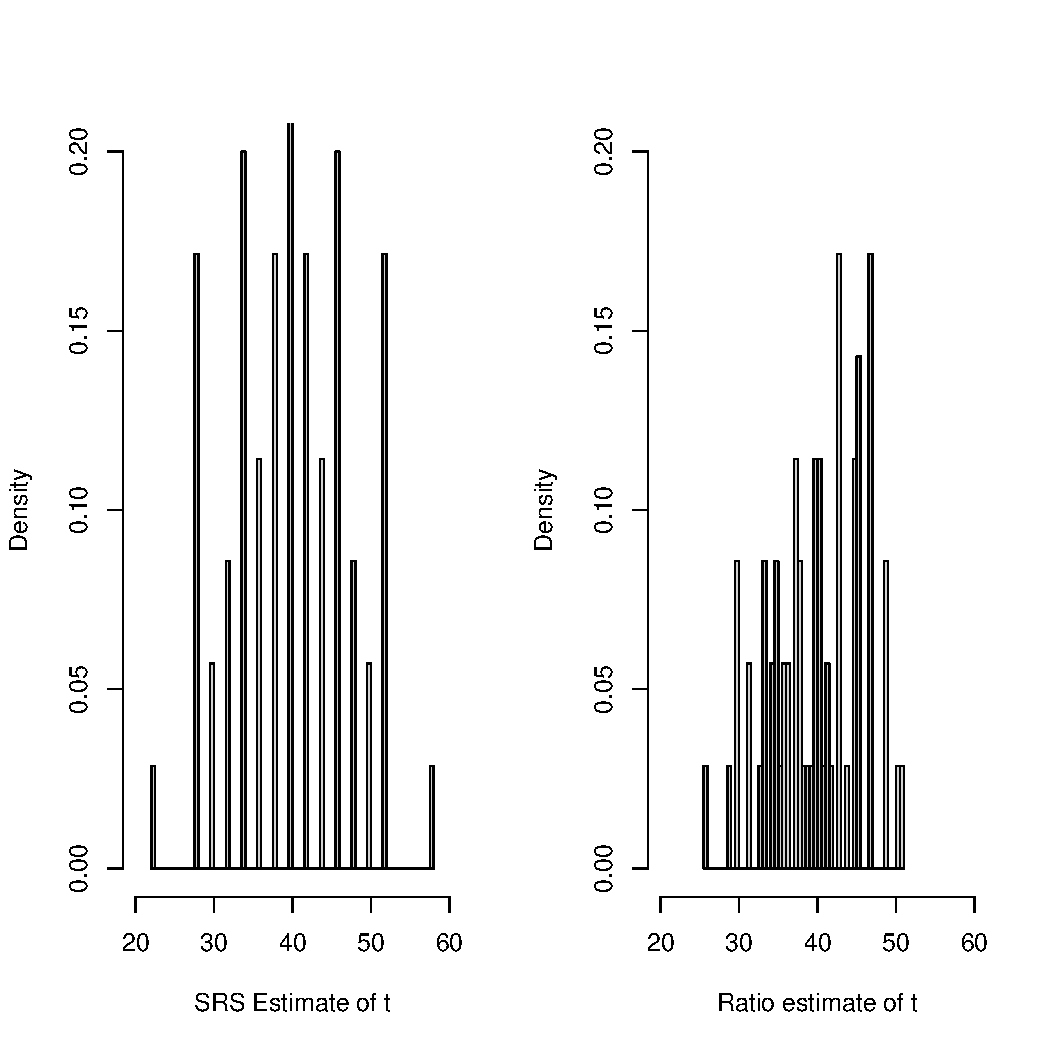
\includegraphics[width=.7\linewidth]{figure/unnamed-chunk-25-1} 

}


\end{knitrout}
\end{center}
\end{frame}


\subsection{Ratio Estimation with Proportions}
\begin{frame}{}
\begin{block}{}
\begin{center}
Ratio Estimation with Proportions
\end{center}
\end{block}
\end{frame}

\begin{frame}{Ratio Estimation with Proportions}
\begin{block}{}
Ratio estimation works the exactly same way when the quantity of interest is a proportion!
\end{block}
\end{frame}

\begin{frame}{Ratio Estimation with Proportions}
\begin{block}{Example: Feral pigs and Vegetation}
\small
\begin{itemize}
\item Peart (1994) collected the data shown (next slide) as part of a study evaluating the effects of feral pig activity and drought on the native vegetation on Santa Cruz Island, CA.
\item She counted the number of woody seedlings in pig-protected areas under each of ten sampled oak trees in March 1992, following the drought-ending rains of 1991.
\item She put a flag by each seedling, then determined how many were still alive in February 1994. 
\item One naively calculates the error like it was an SRS when wants to find the sample proportion of the 1992 seedlings that are still alive in 1994.
\item This results in SD $\sqrt{(0.2961)(0.7039)/206}=0.0318.$
\item This calculation is incorrect for these data since plots, not individual seedlings, are the sampling units.
\item Technically this design is \textbf{cluster sample}.
\end{itemize}
\end{block}
\end{frame}

\begin{frame}[containsverbatim]{Ratio Estimation with Proportions}
\small
\begin{knitrout}
\definecolor{shadecolor}{rgb}{1, 1, 1}\color{fgcolor}\begin{kframe}
\begin{alltt}
\hlstd{scIsland} \hlkwb{<-} \hlkwd{data.frame}\hlstd{(}\hlkwc{Tree} \hlstd{=} \hlnum{1}\hlopt{:}\hlnum{10}\hlstd{,} \hlkwc{x} \hlstd{=} \hlkwd{c}\hlstd{(}\hlnum{1}\hlstd{,}
    \hlnum{0}\hlstd{,} \hlnum{8}\hlstd{,} \hlnum{2}\hlstd{,} \hlnum{76}\hlstd{,} \hlnum{60}\hlstd{,} \hlnum{25}\hlstd{,} \hlnum{2}\hlstd{,} \hlnum{1}\hlstd{,} \hlnum{31}\hlstd{),} \hlkwc{y} \hlstd{=} \hlkwd{c}\hlstd{(}\hlnum{0}\hlstd{,}
    \hlnum{0}\hlstd{,} \hlnum{1}\hlstd{,} \hlnum{2}\hlstd{,} \hlnum{10}\hlstd{,} \hlnum{15}\hlstd{,} \hlnum{3}\hlstd{,} \hlnum{2}\hlstd{,} \hlnum{1}\hlstd{,} \hlnum{27}\hlstd{))}

\hlkwd{mean}\hlstd{(scIsland}\hlopt{$}\hlstd{x)}
\end{alltt}
\begin{verbatim}
 R >  [1] 20.6
\end{verbatim}
\begin{alltt}
\hlkwd{sd}\hlstd{(scIsland}\hlopt{$}\hlstd{x)}
\end{alltt}
\begin{verbatim}
 R >  [1] 27.47201
\end{verbatim}
\begin{alltt}
\hlkwd{mean}\hlstd{(scIsland}\hlopt{$}\hlstd{y)}
\end{alltt}
\begin{verbatim}
 R >  [1] 6.1
\end{verbatim}
\begin{alltt}
\hlkwd{sd}\hlstd{(scIsland}\hlopt{$}\hlstd{y)}
\end{alltt}
\begin{verbatim}
 R >  [1] 8.824839
\end{verbatim}
\end{kframe}
\end{knitrout}

\end{frame}

\begin{frame}[containsverbatim]{Ratio Estimation with Proportions}
\tiny
\begin{knitrout}
\definecolor{shadecolor}{rgb}{1, 1, 1}\color{fgcolor}\begin{kframe}
\begin{alltt}
\hlkwd{plot}\hlstd{(scIsland}\hlopt{$}\hlstd{x, scIsland}\hlopt{$}\hlstd{y,} \hlkwc{pch} \hlstd{=} \hlnum{19}\hlstd{,} \hlkwc{xlab} \hlstd{=} \hlstr{"Seedlings Alive *March 1992)"}\hlstd{,}
    \hlkwc{ylab} \hlstd{=} \hlstr{"Seedlings that Survived (February 1994)"}\hlstd{,}
    \hlkwc{xlim} \hlstd{=} \hlkwd{c}\hlstd{(}\hlopt{-}\hlnum{1}\hlstd{,} \hlnum{80}\hlstd{),} \hlkwc{ylim} \hlstd{=} \hlkwd{c}\hlstd{(}\hlopt{-}\hlnum{1}\hlstd{,} \hlnum{30}\hlstd{))}
\hlstd{l} \hlkwb{<-} \hlstd{lm} \hlkwb{<-} \hlkwd{lm}\hlstd{(y} \hlopt{~} \hlstd{x} \hlopt{-} \hlnum{1}\hlstd{,} \hlkwc{data} \hlstd{= scIsland)}
\hlkwd{curve}\hlstd{(}\hlkwd{coef}\hlstd{(l)[}\hlnum{1}\hlstd{]} \hlopt{*} \hlstd{x,} \hlkwc{from} \hlstd{=} \hlopt{-}\hlnum{1}\hlstd{,} \hlkwc{to} \hlstd{=} \hlnum{80}\hlstd{,}
    \hlkwc{add} \hlstd{=} \hlnum{TRUE}\hlstd{)}
\end{alltt}
\end{kframe}

{\centering 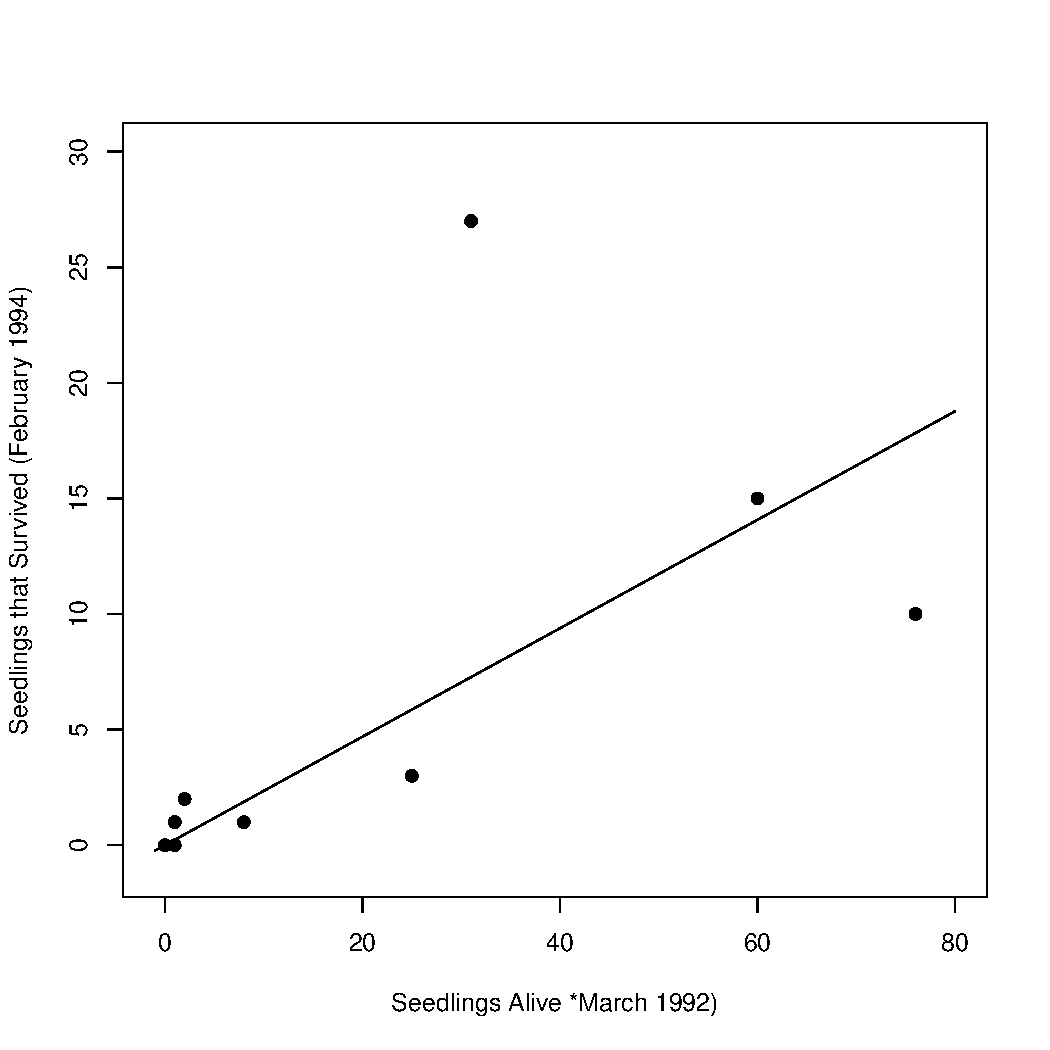
\includegraphics[width=.5\linewidth]{figure/unnamed-chunk-27-1} 

}


\end{knitrout}

\end{frame}

\begin{frame}[containsverbatim]{Ratio Estimation with Proportions}
\small
\begin{knitrout}
\definecolor{shadecolor}{rgb}{1, 1, 1}\color{fgcolor}\begin{kframe}
\begin{alltt}
\hlcom{## Bhat =phat}
\hlstd{Bhat} \hlkwb{<-} \hlkwd{mean}\hlstd{(scIsland}\hlopt{$}\hlstd{y)}\hlopt{/}\hlkwd{mean}\hlstd{(scIsland}\hlopt{$}\hlstd{x)}
\hlstd{se2} \hlkwb{<-} \hlkwd{var}\hlstd{(scIsland}\hlopt{$}\hlstd{y} \hlopt{-} \hlstd{Bhat} \hlopt{*} \hlstd{(scIsland}\hlopt{$}\hlstd{x))}
\hlstd{se.bhat.nfpc} \hlkwb{<-} \hlkwd{sqrt}\hlstd{((}\hlnum{1}\hlopt{/}\hlstd{(}\hlnum{10} \hlopt{*} \hlkwd{mean}\hlstd{(scIsland}\hlopt{$}\hlstd{x)}\hlopt{^}\hlnum{2}\hlstd{))} \hlopt{*}
    \hlstd{se2)}
\hlstd{se.bhat.nfpc}
\end{alltt}
\begin{verbatim}
 R >  [1] 0.1152622
\end{verbatim}
\end{kframe}
\end{knitrout}
\end{frame}

\subsection{Ratio Estimation Using Weight Adjustments}
\begin{frame}{}
\begin{block}{}
\begin{center}
Ratio Estimation Using Weight Adjustments
\end{center}
\end{block}
\end{frame}

\begin{frame}{Ratio Estimation Using Weight Adjustments}
\begin{block}{Weights}
\begin{align*}
w_i &= 1/\pi_i\\
\hat{t}_y &= \sum_{i \in S} w_i y_i\\
\hat{t}_{yr} &= \frac{t_x}{\hat{t}_x}\hat{t}_y = \frac{t_x}{\hat{t}_x} \sum_{i\in S} w_i y_i
\end{align*}
\end{block}
\end{frame}

\begin{frame}{Ratio Estimation Using Weight Adjustments}
\begin{block}{Weights}
We can think of the modification used in ratio estimation as an adjustment to each weight. Define:
\begin{align*}
g_i = \frac{t_x}{\hat{t}_x} \\
\hat{t}_{yr} = \sum_{i \in S} w_i g_i y_i
\end{align*}
\end{block}
\end{frame}


\begin{frame}{Ratio Estimation Using Weight Adjustments}
\begin{block}{Weights}
The estimator $\hat{t}_{yr}$ is a weighted sum of observations, with weight $w_i^* =w_ig_i$. Unlike the original weights $w_i$, however, the adjusted weights $w_i^*$ depend upon values from the sample: If a different sample is taken, the weight adjustment $g_i=t_x/\hat{t}_x$ will be different.
\end{block}
\end{frame}

\begin{frame}{Ratio Estimation Using Weight Adjustments}
\begin{block}{Weights}
The weight adjustment $g_i$ \textbf{calibrate} the estimates on the $x$ variable. Since
\begin{align*}
\sum_{i \in S} w_ig_i x_i = t_x
\end{align*}
the adjusted weights force the estimated total for the $x$ variable to equal the known population total $t_x$. The factors $g_i$ are called the \textbf{calibration factors}.
\end{block}
\end{frame}


\begin{frame}{Ratio Estimation Using Weight Adjustments}
\begin{block}{Weights}
The variance estimators can be calculated by forming the new variable $u_i=g_ie_i$. Then for an SRS
\begin{align*}
\hat{V}(\bar{u}) = \left( 1-\frac{n}{N}\right) \frac{1}{n(n-1)} \sum_{i\in S} (u_i -\bar{u})^2 = \left(1-\frac{n}{N}\right) \frac{s_e^2}{n} \left( \frac{t_x}{\hat{t}_x}\right)^2 = \hat{V}(\hat{\bar{y}}_r)
\end{align*}
Similarly $\hat{V}(\hat{t}_u) = \hat{V}(\hat{t}_{yr})$
\end{block}
\end{frame}

\begin{frame}[containsverbatim]{Ratio Estimation Using Weight Adjustments}
\small
\begin{knitrout}
\definecolor{shadecolor}{rgb}{1, 1, 1}\color{fgcolor}\begin{kframe}
\begin{alltt}
\hlkwd{library}\hlstd{(lohrData)}
\hlkwd{data}\hlstd{(agsrs)}
\hlstd{g} \hlkwb{<-} \hlnum{964470625}\hlopt{/}\hlstd{(}\hlkwd{mean}\hlstd{(agsrs}\hlopt{$}\hlstd{ACRES87)} \hlopt{*} \hlnum{3078}\hlstd{)}  \hlcom{#t_x/hat_t_x}
\hlstd{w} \hlkwb{<-} \hlnum{3078}\hlopt{/}\hlnum{300}
\hlstd{w.star} \hlkwb{<-} \hlstd{w} \hlopt{*} \hlstd{g}
\hlstd{wgx} \hlkwb{<-} \hlstd{w.star} \hlopt{*} \hlstd{agsrs}\hlopt{$}\hlstd{ACRES87}
\hlkwd{sum}\hlstd{(wgx)}  \hlcom{#t_x}
\end{alltt}
\begin{verbatim}
 R >  [1] 964470625
\end{verbatim}
\begin{alltt}
\hlstd{wgy} \hlkwb{<-} \hlstd{w.star} \hlopt{*} \hlstd{agsrs}\hlopt{$}\hlstd{ACRES92}
\hlkwd{sum}\hlstd{(wgy)}  \hlcom{#hat_t_yr}
\end{alltt}
\begin{verbatim}
 R >  [1] 951513191
\end{verbatim}
\begin{alltt}
\hlcom{## Note that sum wg \textbackslash{}neq N=3078}
\hlnum{300} \hlopt{*} \hlstd{w.star}
\end{alltt}
\begin{verbatim}
 R >  [1] 3194.101
\end{verbatim}
\end{kframe}
\end{knitrout}
\end{frame}

\begin{frame}{}
\begin{block}{}
Review of Regression Estimation
\end{block}
\end{frame}

\subsection{Regression Estimation in SRS}


\begin{frame}{Regression Estimation in SRS}
\only<1>{
\begin{block}{The Linear Model: One variable}
$$y=B_o+B_1x$$
Let the estimators for $\hat{B}_0$ and $\hat{B}_1$ be the OLS regression coefficients of the slope and intercept.
\begin{align*}
\hat{B}_1 &= \frac{\sum_{i \in S} (x_i-\bar{x})(y_i-\bar{y})}{\sum_{i \in S} (x_i-\bar{x})^2} = \frac{r s_y}{s_x}\\
\hat{B}_0 &= \bar{y}-\hat{B}_1 \bar{x}
\end{align*} 
where $r$ is the sample correlation coefficient for $x$ and $y$.
\end{block}
}
\only<2>{
\begin{block}{The Linear Model}
\begin{itemize}
\item Regression estimation (similar to ratio estimation) uses the correlation between $x$ and $y$ to obtain an estimator for $\bar{y}_U$ with (hopefully) increased precision.
\item Suppose we know $\bar{x}_U$ the population mean for the $x$'s. Then the regression estimator of $\bar{y}_U$ is the predicted value of $y$ from the fitted regression equation when $x=\bar{x}_U$.
$$\hat{\bar{y}}_{reg} = \hat{B}_0+\hat{B}_1\bar{x}_U = \bar{y}+\hat{B}_1(\bar{x}_U-\bar{x})$$
\begin{itemize}
\item If $\bar{x}$ from the sample is smaller than the population mean $\bar{x}_U$ and $x$ and $y$ are positively correlated, then we would expect $\bar{y}$ to also be smaller then $\bar{y}_U$.
\item The regression estimator adjusts $\bar{y}$ by the quantity $\hat{B}_1(\bar{x}_U-\bar{x})$.
\end{itemize}
\end{itemize}
\end{block}
}
\only<3>{
\begin{block}{The Linear Model}
\begin{itemize}
\item Like the ratio estimator, the regression estimator is biased!
\item Let $B_1$ be the least squares regression slope calculated from all the data in the population.
$$B_1 = \frac{\sum_{i =1}^N (x_i-\bar{x}_U)(y_i-\bar{y}_U)}{\sum_{i =1}^N (x_i-\bar{x}_U)^2} =\frac{RS_y}{S_x}$$
\end{itemize}
\end{block}
}
\only<4>{
\begin{block}{The Linear Model}
\begin{itemize}
\item Bias
\end{itemize}
\end{block}
}
\only<5>{
\begin{block}{The Linear Model}
\begin{itemize}
\item MSE
\end{itemize}
\end{block}
}
\only<6>{
\begin{block}{The Linear Model}
\begin{itemize}
\item The SE can be calculated by substituting estimates for the population quantities. We can estimate $S_d^2$ by using the residuals $e_i=y_i-(\hat{B}_0+\hat{B}_1x_i)$. $s_e^2=\sum_{i \in S} e_i^2/(n-1)$ estimates $S_d^2$ and
$$SE(\hat{\bar{y}}_{reg}) = \sqrt{\left(1-\frac{n}{N}\right)\frac{s_e^2}{n}}$$
\end{itemize}
\end{block}
}

\only<7>{
\begin{block}{The Linear Model}
\begin{itemize}
\item In small samples, we may alternatively calculate $s_e^2$ using the MSE from a regression analysis $$s_e^2 = \sum_{i\in S} e_i^2/(n-2)$$.
\item Where does this come from?
\item To estimate the variance for this formulation
$$SE(\hat{\bar{y}}_{reg}) = \sqrt{\left(1-\frac{n}{N}\right)\frac{1}{n}s_y^2(1-r^2)}$$
\end{itemize}
\end{block}
}
\end{frame}

\subsection{Example: Trees}
\begin{frame}[containsverbatim]{Example: Trees}
\begin{block}{}
\begin{itemize}
\item To estimate the number of dead trees in an area, we divide the area into 100 square plots and count the number of dead trees on a photograph of each plot.
\item Photo counts can be made quickly, but sometimes a tree is misclassified or not detected.
\item So we select an SRS of 25 of the plots for field counts of dead trees (quality control)
\item We know that the population mean number of dead trees per plot from the photo count is 11.3.
\end{itemize}
\end{block}
\end{frame}

\begin{frame}[containsverbatim]{Example: Trees}
\small
\begin{knitrout}
\definecolor{shadecolor}{rgb}{1, 1, 1}\color{fgcolor}\begin{kframe}
\begin{alltt}
\hlstd{photo.x} \hlkwb{<-} \hlkwd{c}\hlstd{(}\hlnum{10}\hlstd{,} \hlnum{12}\hlstd{,} \hlnum{7}\hlstd{,} \hlnum{13}\hlstd{,} \hlnum{13}\hlstd{,} \hlnum{6}\hlstd{,} \hlnum{17}\hlstd{,} \hlnum{16}\hlstd{,}
    \hlnum{15}\hlstd{,} \hlnum{10}\hlstd{,} \hlnum{14}\hlstd{,} \hlnum{12}\hlstd{,} \hlnum{10}\hlstd{,} \hlnum{5}\hlstd{,} \hlnum{12}\hlstd{,} \hlnum{10}\hlstd{,} \hlnum{10}\hlstd{,} \hlnum{9}\hlstd{,}
    \hlnum{6}\hlstd{,} \hlnum{11}\hlstd{,} \hlnum{7}\hlstd{,} \hlnum{9}\hlstd{,} \hlnum{11}\hlstd{,} \hlnum{10}\hlstd{,} \hlnum{10}\hlstd{)}
\hlstd{photo.y} \hlkwb{<-} \hlkwd{c}\hlstd{(}\hlnum{15}\hlstd{,} \hlnum{14}\hlstd{,} \hlnum{9}\hlstd{,} \hlnum{14}\hlstd{,} \hlnum{8}\hlstd{,} \hlnum{5}\hlstd{,} \hlnum{18}\hlstd{,} \hlnum{15}\hlstd{,}
    \hlnum{13}\hlstd{,} \hlnum{15}\hlstd{,} \hlnum{11}\hlstd{,} \hlnum{15}\hlstd{,} \hlnum{12}\hlstd{,} \hlnum{8}\hlstd{,} \hlnum{13}\hlstd{,} \hlnum{9}\hlstd{,} \hlnum{11}\hlstd{,} \hlnum{12}\hlstd{,}
    \hlnum{9}\hlstd{,} \hlnum{12}\hlstd{,} \hlnum{13}\hlstd{,} \hlnum{11}\hlstd{,} \hlnum{10}\hlstd{,} \hlnum{9}\hlstd{,} \hlnum{8}\hlstd{)}
\hlstd{photo} \hlkwb{<-} \hlkwd{data.frame}\hlstd{(}\hlkwc{x} \hlstd{= photo.x,} \hlkwc{y} \hlstd{= photo.y)}
\end{alltt}
\end{kframe}
\end{knitrout}
\end{frame}

\begin{frame}[containsverbatim]{Example: Trees}
\small
\begin{knitrout}
\definecolor{shadecolor}{rgb}{1, 1, 1}\color{fgcolor}\begin{kframe}
\begin{alltt}
\hlstd{desc} \hlkwb{<-} \hlkwd{matrix}\hlstd{(}\hlkwd{c}\hlstd{(}\hlkwd{mean}\hlstd{(photo}\hlopt{$}\hlstd{x),} \hlkwd{mean}\hlstd{(photo}\hlopt{$}\hlstd{y),}
    \hlkwd{sd}\hlstd{(photo}\hlopt{$}\hlstd{x),} \hlkwd{sd}\hlstd{(photo}\hlopt{$}\hlstd{y)),} \hlkwc{byrow} \hlstd{=} \hlnum{FALSE}\hlstd{,}
    \hlkwc{nc} \hlstd{=} \hlnum{2}\hlstd{,} \hlkwc{dimnames} \hlstd{=} \hlkwd{list}\hlstd{(}\hlkwd{c}\hlstd{(}\hlstr{"x"}\hlstd{,} \hlstr{"y"}\hlstd{),}
        \hlkwd{c}\hlstd{(}\hlstr{"Mean"}\hlstd{,} \hlstr{"SD"}\hlstd{)))}
\hlstd{desc}
\end{alltt}
\begin{verbatim}
 R >     Mean       SD
 R >  x 10.60 3.068659
 R >  y 11.56 3.014963
\end{verbatim}
\begin{alltt}
\hlkwd{cor}\hlstd{(photo}\hlopt{$}\hlstd{x, photo}\hlopt{$}\hlstd{y)}
\end{alltt}
\begin{verbatim}
 R >  [1] 0.6241967
\end{verbatim}
\end{kframe}
\end{knitrout}
\end{frame}

\begin{frame}[containsverbatim]{Example: Trees}
\small
\begin{knitrout}
\definecolor{shadecolor}{rgb}{1, 1, 1}\color{fgcolor}\begin{kframe}
\begin{alltt}
\hlkwd{plot}\hlstd{(photo}\hlopt{$}\hlstd{x, photo}\hlopt{$}\hlstd{y,} \hlkwc{pch} \hlstd{=} \hlnum{19}\hlstd{,} \hlkwc{cex} \hlstd{=} \hlnum{0.5}\hlstd{,}
    \hlkwc{xlab} \hlstd{=} \hlstr{"Photo of Dead Trees"}\hlstd{,} \hlkwc{ylab} \hlstd{=} \hlstr{"Field Count of Dead Trees"}\hlstd{)}
\hlstd{l} \hlkwb{<-} \hlkwd{lm}\hlstd{(y} \hlopt{~} \hlstd{x,} \hlkwc{data} \hlstd{= photo)}
\hlkwd{curve}\hlstd{(}\hlkwd{coef}\hlstd{(l)[}\hlnum{1}\hlstd{]} \hlopt{+} \hlkwd{coef}\hlstd{(l)[}\hlnum{2}\hlstd{]} \hlopt{*} \hlstd{x,} \hlkwc{from} \hlstd{=} \hlkwd{min}\hlstd{(photo),}
    \hlkwc{to} \hlstd{=} \hlkwd{max}\hlstd{(photo),} \hlkwc{add} \hlstd{=} \hlnum{TRUE}\hlstd{)}
\end{alltt}
\end{kframe}
\end{knitrout}
\end{frame}

\begin{frame}[containsverbatim]{Example: Trees}
\small

\begin{center}
\vspace{-.3in}
\begin{knitrout}
\definecolor{shadecolor}{rgb}{1, 1, 1}\color{fgcolor}

{\centering 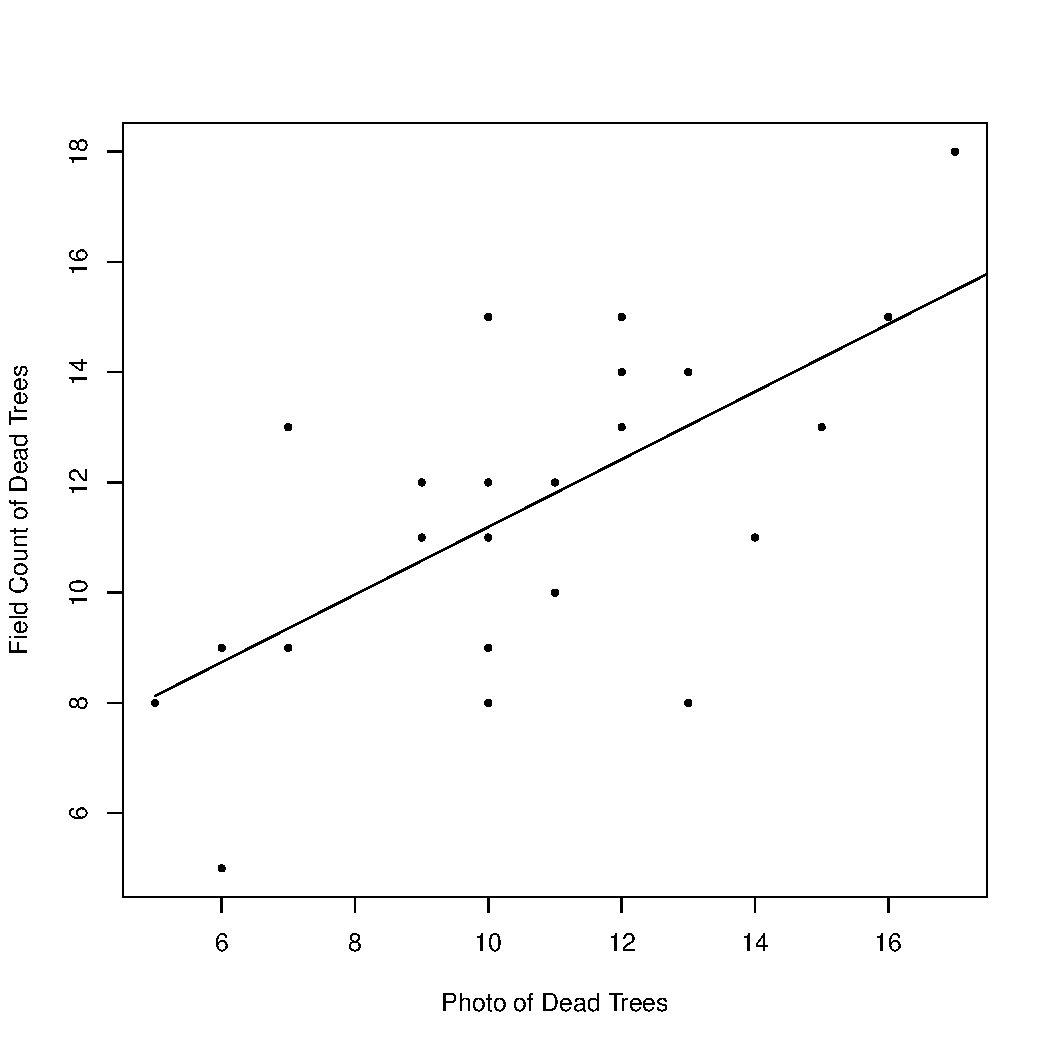
\includegraphics[width=.7\linewidth]{figure/unnamed-chunk-33-1} 

}


\end{knitrout}
\end{center}
\end{frame}

\begin{frame}[containsverbatim]{Example: Trees}
\begin{block}{}
$$\hat{y}= 5.059292+0.613274x$$
\end{block}

\begin{itemize}
\item $\hat{B}_0 = 5.059292$
\item $\hat{B}_1 = 0.613274$
\item x and y are positively correlated so that $\bar{x}$ and $\bar{y}$ are also positively correlated.
\item Since $\bar{x}<\bar{x}_U$, we expect $$\hat{B}_1(\bar{x}_U-\bar{x}) = 0.613274(11.3-10.6) =0.43$$
to $\bar{y}$ to compensate.
\end{itemize}


\end{frame}

\begin{frame}[containsverbatim]{Example: Trees}
\begin{block}{}
$$\hat{y}= 5.059292+0.613274x$$
\end{block}

\begin{itemize}
\item The regression estimate of the mean is
$$\hat{y}= 5.059292+0.613274 11.3 = 11.99$$
\end{itemize}


\end{frame}

\begin{frame}[containsverbatim]{Example: Trees}
\begin{knitrout}
\definecolor{shadecolor}{rgb}{1, 1, 1}\color{fgcolor}\begin{kframe}
\begin{alltt}
\hlstd{se.yreg} \hlkwb{<-} \hlkwd{sqrt}\hlstd{((}\hlnum{1} \hlopt{-} \hlkwd{length}\hlstd{(photo}\hlopt{$}\hlstd{y)}\hlopt{/}\hlnum{100}\hlstd{)} \hlopt{*}
    \hlstd{(}\hlkwd{var}\hlstd{(photo}\hlopt{$}\hlstd{y)}\hlopt{/}\hlnum{25}\hlstd{)} \hlopt{*} \hlstd{(}\hlnum{1} \hlopt{-} \hlkwd{cor}\hlstd{(photo}\hlopt{$}\hlstd{y,}
    \hlstd{photo}\hlopt{$}\hlstd{x)}\hlopt{^}\hlnum{2}\hlstd{))}
\hlstd{se.yreg}
\end{alltt}
\begin{verbatim}
 R >  [1] 0.4079831
\end{verbatim}
\end{kframe}
\end{knitrout}
Compare to
\begin{knitrout}
\definecolor{shadecolor}{rgb}{1, 1, 1}\color{fgcolor}\begin{kframe}
\begin{alltt}
\hlstd{se.ybar} \hlkwb{<-} \hlkwd{sqrt}\hlstd{((}\hlnum{1} \hlopt{-} \hlkwd{length}\hlstd{(photo}\hlopt{$}\hlstd{y)}\hlopt{/}\hlnum{100}\hlstd{)} \hlopt{*}
    \hlstd{(}\hlkwd{var}\hlstd{(photo}\hlopt{$}\hlstd{y)}\hlopt{/}\hlnum{25}\hlstd{))}
\hlstd{se.ybar}
\end{alltt}
\begin{verbatim}
 R >  [1] 0.5222069
\end{verbatim}
\end{kframe}
\end{knitrout}
\end{frame}

\begin{frame}[containsverbatim]{Example: Trees}
We expect the regression estimator to increase the precision in this example b/c the variables photo and field are positively correlated. To estimate the total number of dead trees, use
\begin{knitrout}
\definecolor{shadecolor}{rgb}{1, 1, 1}\color{fgcolor}\begin{kframe}
\begin{alltt}
\hlstd{t_reg} \hlkwb{<-} \hlnum{100} \hlopt{*} \hlstd{(}\hlkwd{coef}\hlstd{(l)[}\hlnum{1}\hlstd{]} \hlopt{+} \hlkwd{coef}\hlstd{(l)[}\hlnum{2}\hlstd{]} \hlopt{*}
    \hlnum{11.3}\hlstd{)}
\hlstd{t_reg}
\end{alltt}
\begin{verbatim}
 R >  (Intercept) 
 R >     1198.929
\end{verbatim}
\begin{alltt}
\hlstd{se.treg} \hlkwb{<-} \hlnum{100} \hlopt{*} \hlstd{se.yreg}
\hlstd{se.treg}
\end{alltt}
\begin{verbatim}
 R >  [1] 40.79831
\end{verbatim}
\end{kframe}
\end{knitrout}
\end{frame}



\subsection{Difference Estimation}

\begin{frame}{}
\begin{block}{}
\begin{center}
Difference Estimation
\end{center}
\end{block}

\end{frame}

\begin{frame}{Difference Estimation}
\begin{block}{}
\textbf{Difference Estimation} is a special case of regression estimation, used when the investigator ``knows" that the slope $B_1=1$.
\end{block}
\end{frame}

\begin{frame}{Difference Estimation}
\begin{block}{}
\begin{itemize}
\item Difference estimation is often recommended in accounting when an SRS is taken.
\item A list of accounts receivable consists of the book value for each account -- the company's listing of how much is owed on each account.
\item In the simplest sampling scheme, the auditor scrutinizes a random sample of the accounts to determine the audited value (actual amount owed).
\item The quantities considered

\begin{align*}
y_i &= \textrm{ audited value for company $i$}\\
x_i &= \textrm{ book value for company $i$}
\end{align*}

Then, $\bar{y}-\bar{x}$ is the mean difference for the audited accounts.
\end{itemize}
\end{block}
\end{frame}

\begin{frame}{Difference Estimation}
\begin{block}{}
\begin{itemize}
\item The estimated total difference is $$\hat{t}_y-\hat{t}_x=N(\bar{y}-\bar{x})$$
\item The estimated audited value for accounts receivable is thus
$$\hat{t}_{ydiff} = t_x-(\hat{t}_y-\hat{t}_x)$$
\item The residuals from this model are $e_i = y_i-x_i$. The variance of $\hat{t}_{ydiff}$ is
$$V(\hat{t}_{ydiff})= V[ t_x-(\hat{t}_y-\hat{t}_x] = V(\hat{t}_e)$$
where $\hat{t}_e = (N/n)\sum_{i \in S} e_i$.
\end{itemize}
\end{block}
\end{frame}

\begin{frame}{Difference Estimation}
\begin{block}{}
\begin{itemize}
\item Difference estimation works best if the population and sample have a larger fraction of nonzero differences that are roughly equally divided between overstatements and understatements.
\item If the sample is large enough so that the sampling distribution of $(\bar{y}-\bar{x})$ is approximately normal.
\item Often in the real case of auditing one would want to use a more stable model based estimate.
\end{itemize}
\end{block}
\end{frame}

\subsection{Poststratification}
\begin{frame}{}
\begin{block}{}
\begin{center}
Poststratification
\end{center}
\end{block}
\end{frame}

\begin{frame}{Poststratification}
\begin{block}{Motivation}
\begin{itemize}
\item Earlier in the course we showed the increase in precision that can come from using population data to stratify.
\item \underline{Stratification} is not always a desirable way to use these population data!
\item There may be too many potential stratification variables.
\item The need for cluster sampling may prevent stratification on individual-level variables.
\item Population data may also be available in a form that does not allow for stratification (e.g., random digit dialing).
\item Poststratification is a technique for using known population totals for a set of variables to adjust the sampling weights and improve estimation for another set of variables.
\end{itemize}
\end{block}
\end{frame}

\begin{frame}{Poststratification}
\begin{block}{Motivation}
\begin{itemize}
\item All of the techniques we will discuss have the same idea: adjustments are made to the sampling weights so that estimated population totals for the auxiliary variables match the known population totals, making the sample more representative of the population.
\item A second benefit is that the estimates are forced to be consistent with the population data.
\item This often improves their credibility with people who may not understand the sampling process.
\end{itemize}
\end{block}
\end{frame}


\begin{frame}{Poststratification}
\only<1-2>{
\begin{block}{Motivation}
\begin{itemize}
\item Two core applications of these techniques:
\begin{itemize}
\item Increase precision of estimation.
\item Reduce the bias from nonresponse (especially unit non-response), where a sampled individual refuses to participate or otherwise provides no information for analysis.
\end{itemize}
\end{itemize}
\end{block}
}
\only<2>{
\begin{block}{}
Generally, the use for non-response is considered the more important of the two in large-scale surveys.
\vspace{.2in}

However, this stage is often completed before being handed off to the typical user (e.g., GSS).
\end{block}
}
\end{frame}


\begin{frame}{Poststratification: Example}
\begin{block}{Poststratification by Sex}
The post-stratified estimate of the proportion of Minnesota residents over the age of
18 who are in favor of public funding of the Viking Stadium, $\hat{p}_{post}$ (where the subscript
post denotes ?post-stratified?), is:
\begin{align*}
\hat{p}_{post} &= \frac{N_f}{N}\hat{p}_f+\frac{N_m}{N} \hat{p}_m\\
&= \frac{64,398}{123,516}23.5+\frac{59,118}{123,516}31.1\\
&= 27.16
\end{align*}
\end{block}
\end{frame}


\begin{frame}{Poststratification: Example}
\only<1>{
\begin{block}{Review Stratified Notation}
\begin{align*}
y_{hj} &= \textrm{ the value of the $j$th unit in stratum $h$}\\
t_{h} &= \sum_{j=1}^{N_h} y_{hj} = \textrm{ the population total in stratum $h$}\\
t &= \sum_{h=1}^H t_h = \textrm{ the population total}
\end{align*}
\end{block}
}
\only<2>{
\begin{block}{Mean}
Remember: $$\bar{y}_h=\frac{\sum_{j \in S_h} y_{hj}}{n_h}$$
and the post stratified estimate of the overall sample mean will be
$$\bar{y}_{post} = \sum_{h=1}^H \frac{N_h}{N} \bar{y}_h$$
\end{block}
}

\end{frame}


\begin{frame}{Poststratification}
\begin{block}{Relationship to Ratio Estimation}
\begin{itemize}
\item Define $x_{ih}=1$ if the observation $i$ is in post stratum $h$ and 0 otherwise.
\item Let $u_{ih}=y_i \cdot x_{ih}$.
\item Then $t_{xh} = \sum_{i=1}^N x_{ih}=N_h$ 
\item $t_{uh} = \sum_{i=1}^N u_{ih}$ = population total of variable $y$ in poststratum $h$.
\item $\hat{t}_{uh} = \sum_{i \in S} \frac{N}{n} u_{ih}$
\item We can then use ratio estimation to obtain:
\item $\hat{t}_{uhr} = \frac{t_{xh}}{\hat{t}_{xh}}\hat{t}_{uh}= \frac{N_h}{\hat{N}_h}\hat{t}_{uh} = N_h\bar{y}_h$
\item $\hat{t}_{ypost} = \sum_{h=1}^H \hat{t}_{uhr} = \sum_{h=1}^H \frac{N_h}{\hat{N}_h}\hat{t}_{uh} = \sum_{h=1}^H N_h\bar{y}_h$
\item $\bar{y}_{post} = \sum_{h=1}^H \frac{N_h}{N}\bar{y}_h$
\item $\hat{V}(\bar{y}_{post}) \approx \left(1-\frac{n}{N}\right) \sum_{h=1}^H \frac{N_h}{N} \frac{s_h^2}{n}$
\end{itemize}
\end{block}
\end{frame}

\begin{frame}[containsverbatim]{Poststratification: R Code Example}
\small
\begin{knitrout}
\definecolor{shadecolor}{rgb}{1, 1, 1}\color{fgcolor}\begin{kframe}
\begin{alltt}
\hlkwd{set.seed}\hlstd{(}\hlnum{34567}\hlstd{)}
\hlstd{pop1} \hlkwb{<-} \hlkwd{rpois}\hlstd{(}\hlnum{1000}\hlstd{,} \hlnum{5}\hlstd{)}
\hlstd{pop2} \hlkwb{<-} \hlkwd{rpois}\hlstd{(}\hlnum{5000}\hlstd{,} \hlnum{10}\hlstd{)}
\hlstd{pop} \hlkwb{<-} \hlkwd{c}\hlstd{(pop1, pop2)}
\hlstd{s} \hlkwb{<-} \hlkwd{sample}\hlstd{(}\hlnum{1}\hlopt{:}\hlkwd{length}\hlstd{(pop),} \hlnum{300}\hlstd{)}
\hlstd{y} \hlkwb{<-} \hlstd{pop[s]}
\hlcom{#### Post stratification estimator}
\hlstd{x1} \hlkwb{<-} \hlkwd{as.numeric}\hlstd{(s} \hlopt{<=} \hlnum{1000}\hlstd{)}
\hlstd{x2} \hlkwb{<-} \hlkwd{as.numeric}\hlstd{(s} \hlopt{>} \hlnum{1000}\hlstd{)}
\end{alltt}
\end{kframe}
\end{knitrout}
\end{frame}

\begin{frame}[containsverbatim]{Poststratification: R Code Example}
\small
\begin{knitrout}
\definecolor{shadecolor}{rgb}{1, 1, 1}\color{fgcolor}\begin{kframe}
\begin{alltt}
\hlkwd{table}\hlstd{(x1)}
\end{alltt}
\begin{verbatim}
 R >  x1
 R >    0   1 
 R >  251  49
\end{verbatim}
\begin{alltt}
\hlkwd{table}\hlstd{(x2)}
\end{alltt}
\begin{verbatim}
 R >  x2
 R >    0   1 
 R >   49 251
\end{verbatim}
\begin{alltt}
\hlcom{## Check}
\hlkwd{sum}\hlstd{(x1} \hlopt{+} \hlstd{x2)} \hlopt{==} \hlnum{300}
\end{alltt}
\begin{verbatim}
 R >  [1] TRUE
\end{verbatim}
\end{kframe}
\end{knitrout}
\end{frame}

\begin{frame}[containsverbatim]{Poststratification: R Code Example}
\small
\begin{knitrout}
\definecolor{shadecolor}{rgb}{1, 1, 1}\color{fgcolor}\begin{kframe}
\begin{alltt}
\hlcom{### Build u}
\hlstd{u1} \hlkwb{<-} \hlstd{y} \hlopt{*} \hlstd{x1}
\hlstd{u2} \hlkwb{<-} \hlstd{y} \hlopt{*} \hlstd{x2}

\hlstd{N1} \hlkwb{<-} \hlnum{1000}
\hlstd{N2} \hlkwb{<-} \hlnum{5000}

\hlstd{tu1_hat} \hlkwb{<-} \hlstd{(}\hlnum{6000}\hlopt{/}\hlnum{300}\hlstd{)} \hlopt{*} \hlkwd{sum}\hlstd{(u1)}
\hlstd{tu1_hat}
\end{alltt}
\begin{verbatim}
 R >  [1] 4760
\end{verbatim}
\begin{alltt}
\hlstd{tu2_hat} \hlkwb{<-} \hlstd{(}\hlnum{6000}\hlopt{/}\hlnum{300}\hlstd{)} \hlopt{*} \hlkwd{sum}\hlstd{(u2)}
\hlstd{tu2_hat}
\end{alltt}
\begin{verbatim}
 R >  [1] 51480
\end{verbatim}
\end{kframe}
\end{knitrout}
\end{frame}


\begin{frame}[containsverbatim]{Poststratification: R Code Example}
\small
\begin{knitrout}
\definecolor{shadecolor}{rgb}{1, 1, 1}\color{fgcolor}\begin{kframe}
\begin{alltt}
\hlstd{N1_hat} \hlkwb{<-} \hlnum{6000} \hlopt{*} \hlkwd{mean}\hlstd{(x1)}
\hlstd{N1_hat}
\end{alltt}
\begin{verbatim}
 R >  [1] 980
\end{verbatim}
\begin{alltt}
\hlstd{N2_hat} \hlkwb{<-} \hlnum{6000} \hlopt{*} \hlkwd{mean}\hlstd{(x2)}
\hlstd{N2_hat}
\end{alltt}
\begin{verbatim}
 R >  [1] 5020
\end{verbatim}
\begin{alltt}
\hlstd{t_ypost} \hlkwb{<-} \hlstd{(}\hlnum{1000}\hlopt{/}\hlstd{N1_hat)} \hlopt{*} \hlstd{tu1_hat} \hlopt{+} \hlstd{(}\hlnum{5000}\hlopt{/}\hlstd{N2_hat)} \hlopt{*}
    \hlstd{tu2_hat}
\hlstd{t_ypost}
\end{alltt}
\begin{verbatim}
 R >  [1] 56132.04
\end{verbatim}
\begin{alltt}
\hlstd{t_srs} \hlkwb{<-} \hlnum{6000} \hlopt{*} \hlkwd{mean}\hlstd{(y)}
\hlstd{t_srs}
\end{alltt}
\begin{verbatim}
 R >  [1] 56240
\end{verbatim}
\end{kframe}
\end{knitrout}
\end{frame}


\begin{frame}[containsverbatim]{Poststratification: R Code Example}
\small
\begin{knitrout}
\definecolor{shadecolor}{rgb}{1, 1, 1}\color{fgcolor}\begin{kframe}
\begin{alltt}
\hlstd{ybar.post} \hlkwb{<-} \hlstd{(}\hlnum{1000}\hlopt{/}\hlnum{6000}\hlstd{)} \hlopt{*} \hlkwd{mean}\hlstd{(y[x1} \hlopt{==} \hlnum{1}\hlstd{])} \hlopt{+}
    \hlstd{(}\hlnum{5000}\hlopt{/}\hlnum{6000}\hlstd{)} \hlopt{*} \hlkwd{mean}\hlstd{(y[x2} \hlopt{==} \hlnum{1}\hlstd{])}
\hlstd{ybar.post}
\end{alltt}
\begin{verbatim}
 R >  [1] 9.355341
\end{verbatim}
\begin{alltt}
\hlstd{t_ypost}\hlopt{/}\hlnum{6000}
\end{alltt}
\begin{verbatim}
 R >  [1] 9.355341
\end{verbatim}
\begin{alltt}
\hlstd{y.srs} \hlkwb{<-} \hlkwd{mean}\hlstd{(y)}
\hlstd{y.srs}
\end{alltt}
\begin{verbatim}
 R >  [1] 9.373333
\end{verbatim}
\end{kframe}
\end{knitrout}
\end{frame}

\begin{frame}[containsverbatim]{Poststratification: R Code Example}
\small
\begin{knitrout}
\definecolor{shadecolor}{rgb}{1, 1, 1}\color{fgcolor}\begin{kframe}
\begin{alltt}
\hlstd{s1} \hlkwb{<-} \hlkwd{sd}\hlstd{(y[x1} \hlopt{==} \hlnum{1}\hlstd{])}
\hlstd{s2} \hlkwb{<-} \hlkwd{sd}\hlstd{(y[x2} \hlopt{==} \hlnum{1}\hlstd{])}

\hlstd{v.ybar.post} \hlkwb{<-} \hlstd{(}\hlnum{1} \hlopt{-} \hlnum{300}\hlopt{/}\hlnum{6000}\hlstd{)} \hlopt{*} \hlstd{((}\hlnum{1000}\hlopt{/}\hlnum{6000}\hlstd{)} \hlopt{*}
    \hlstd{s1}\hlopt{^}\hlnum{2}\hlopt{/}\hlnum{300} \hlopt{+} \hlstd{(}\hlnum{5000}\hlopt{/}\hlnum{6000}\hlstd{)} \hlopt{*} \hlstd{s2}\hlopt{^}\hlnum{2}\hlopt{/}\hlnum{300}\hlstd{)}
\hlstd{v.ybar.post}
\end{alltt}
\begin{verbatim}
 R >  [1] 0.03291677
\end{verbatim}
\end{kframe}
\end{knitrout}
\end{frame}









\end{document}
%%%




\section{Sample Size Calculations}
\begin{frame}{Determining Sample Sizes}
\begin{itemize}
\item Assume a stratified sample:
\item $\hat{t}_{yrc} = \hat{B}t_x$
\item $\hat{B} = \frac{\hat{t}_{y,str}}{\hat{t}_{x,str}}$
\item $\hat{t}_{y,str} = \sum_{h=1}^H N_h \bar{y}_h=\sum_{h=1}^H \sum_{j\in S_h} w_{hj}y_{hj}$, where $$w_{hj}=N_h/n_h$
\item $\hat{t}_{x,str} = \sum_{h=1}^H N_h \bar{x}_h=\sum_{h=1}^H \sum_{j\in S_h} w_{hj}x_{hj}$
\end{itemize}

\end{frame}

\begin{frame}[containsverbatim]{}
\small

\end{frame}



%%%%%%%%%%%%
%% Examples
%%%%%%%%%%%%

\begin{frame}{Statistics Review}

\begin{itemize}
\item 
\end{itemize}

\end{frame}


\section{Introduction to R}

\begin{frame}[containsverbatim]{Introduction to R}
\begin{block}{Stuff}
Things
\end{block}
\end{frame}

\begin{frame}[containsverbatim]{R Code Example}
\begin{knitrout}
\definecolor{shadecolor}{rgb}{1, 1, 1}\color{fgcolor}\begin{kframe}
\begin{alltt}
\hlnum{1} \hlopt{+} \hlnum{1}
\end{alltt}
\begin{verbatim}
 R >  [1] 2
\end{verbatim}
\end{kframe}
\end{knitrout}
\end{frame}

%----------- slide --------------------------------------------------%
\begin{frame}[t]{Road Map}

\begin{textblock*}{100mm}(20mm,0.3\textheight)
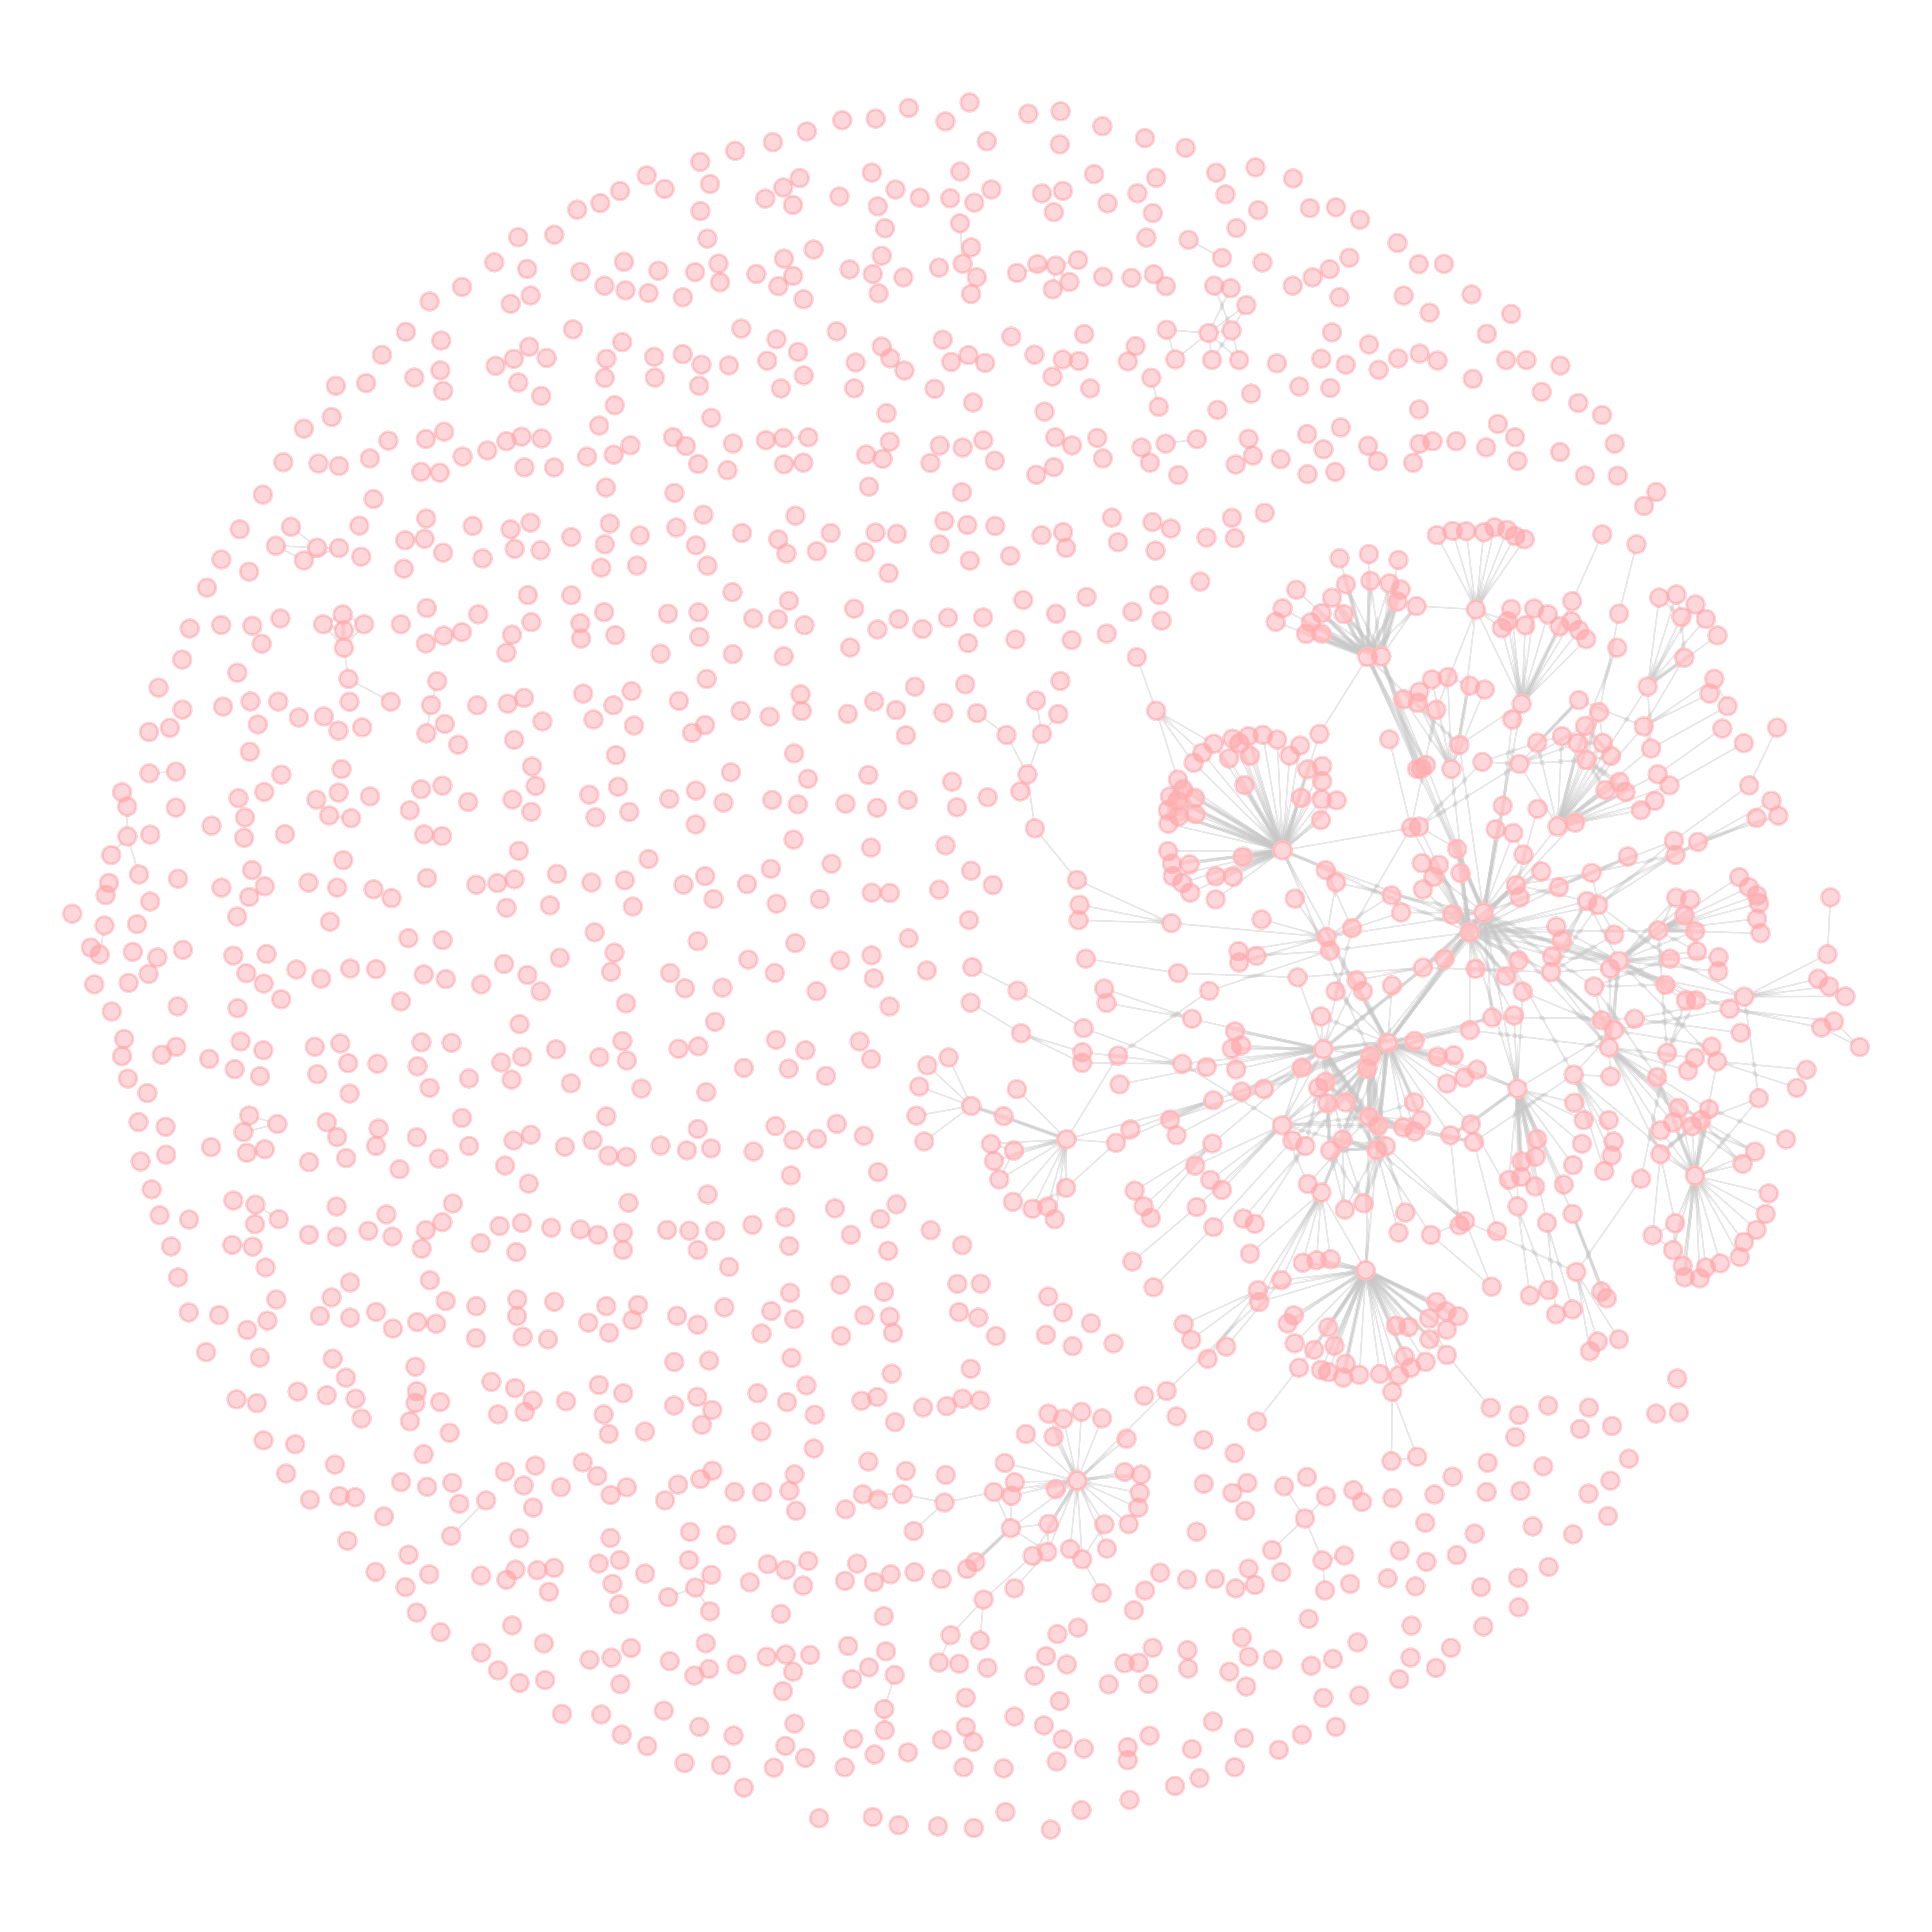
\includegraphics[width=\paperwidth]{graphics/katrinaplot.png}
\end{textblock*}

\begin{textblock*}{100mm}(20mm,0.3\textheight)
\begin{center}
\begin{itemize}
\item[\textbf{1)}] Overview of TERGM with \& w/o vertex dynamics
\begin{itemize}
\item Dynamic network logistic regression w/ \& w/o vertex dynamics
\end{itemize}
\item[\textbf{2)}] Bayesian TERGM 
\begin{itemize}
\item Bayesian analysis of DNR w/ \& w/o vertex dynamics
\end{itemize}
\item[\textbf{3)}] Empirical test cases
\begin{itemize}
\item DNC-RNC blog citation network
\item Lin Freeman's windsurfer network
\end{itemize}
\end{itemize}
\end{center}
\end{textblock*}

%----------- Fix name --------------------------------------------------%
\begin{textblock*}{100mm}(4mm,1.02\textheight)

\includegraphics[width=20mm,heighth=5mm ]{graphics/white.png}
\end{textblock*}

\begin{textblock*}{100mm}(4mm,1.02\textheight)
\emph{\tiny{\darkblue{Zack W Almquist, Sociology and Statistics, UMN}}}
\end{textblock*}
%----------- Fix name --------------------------------------------------%

\end{frame}



%----------- slide --------------------------------------------------%
\begin{frame}[t]{Road Map}

\begin{textblock*}{100mm}(20mm,0.3\textheight)
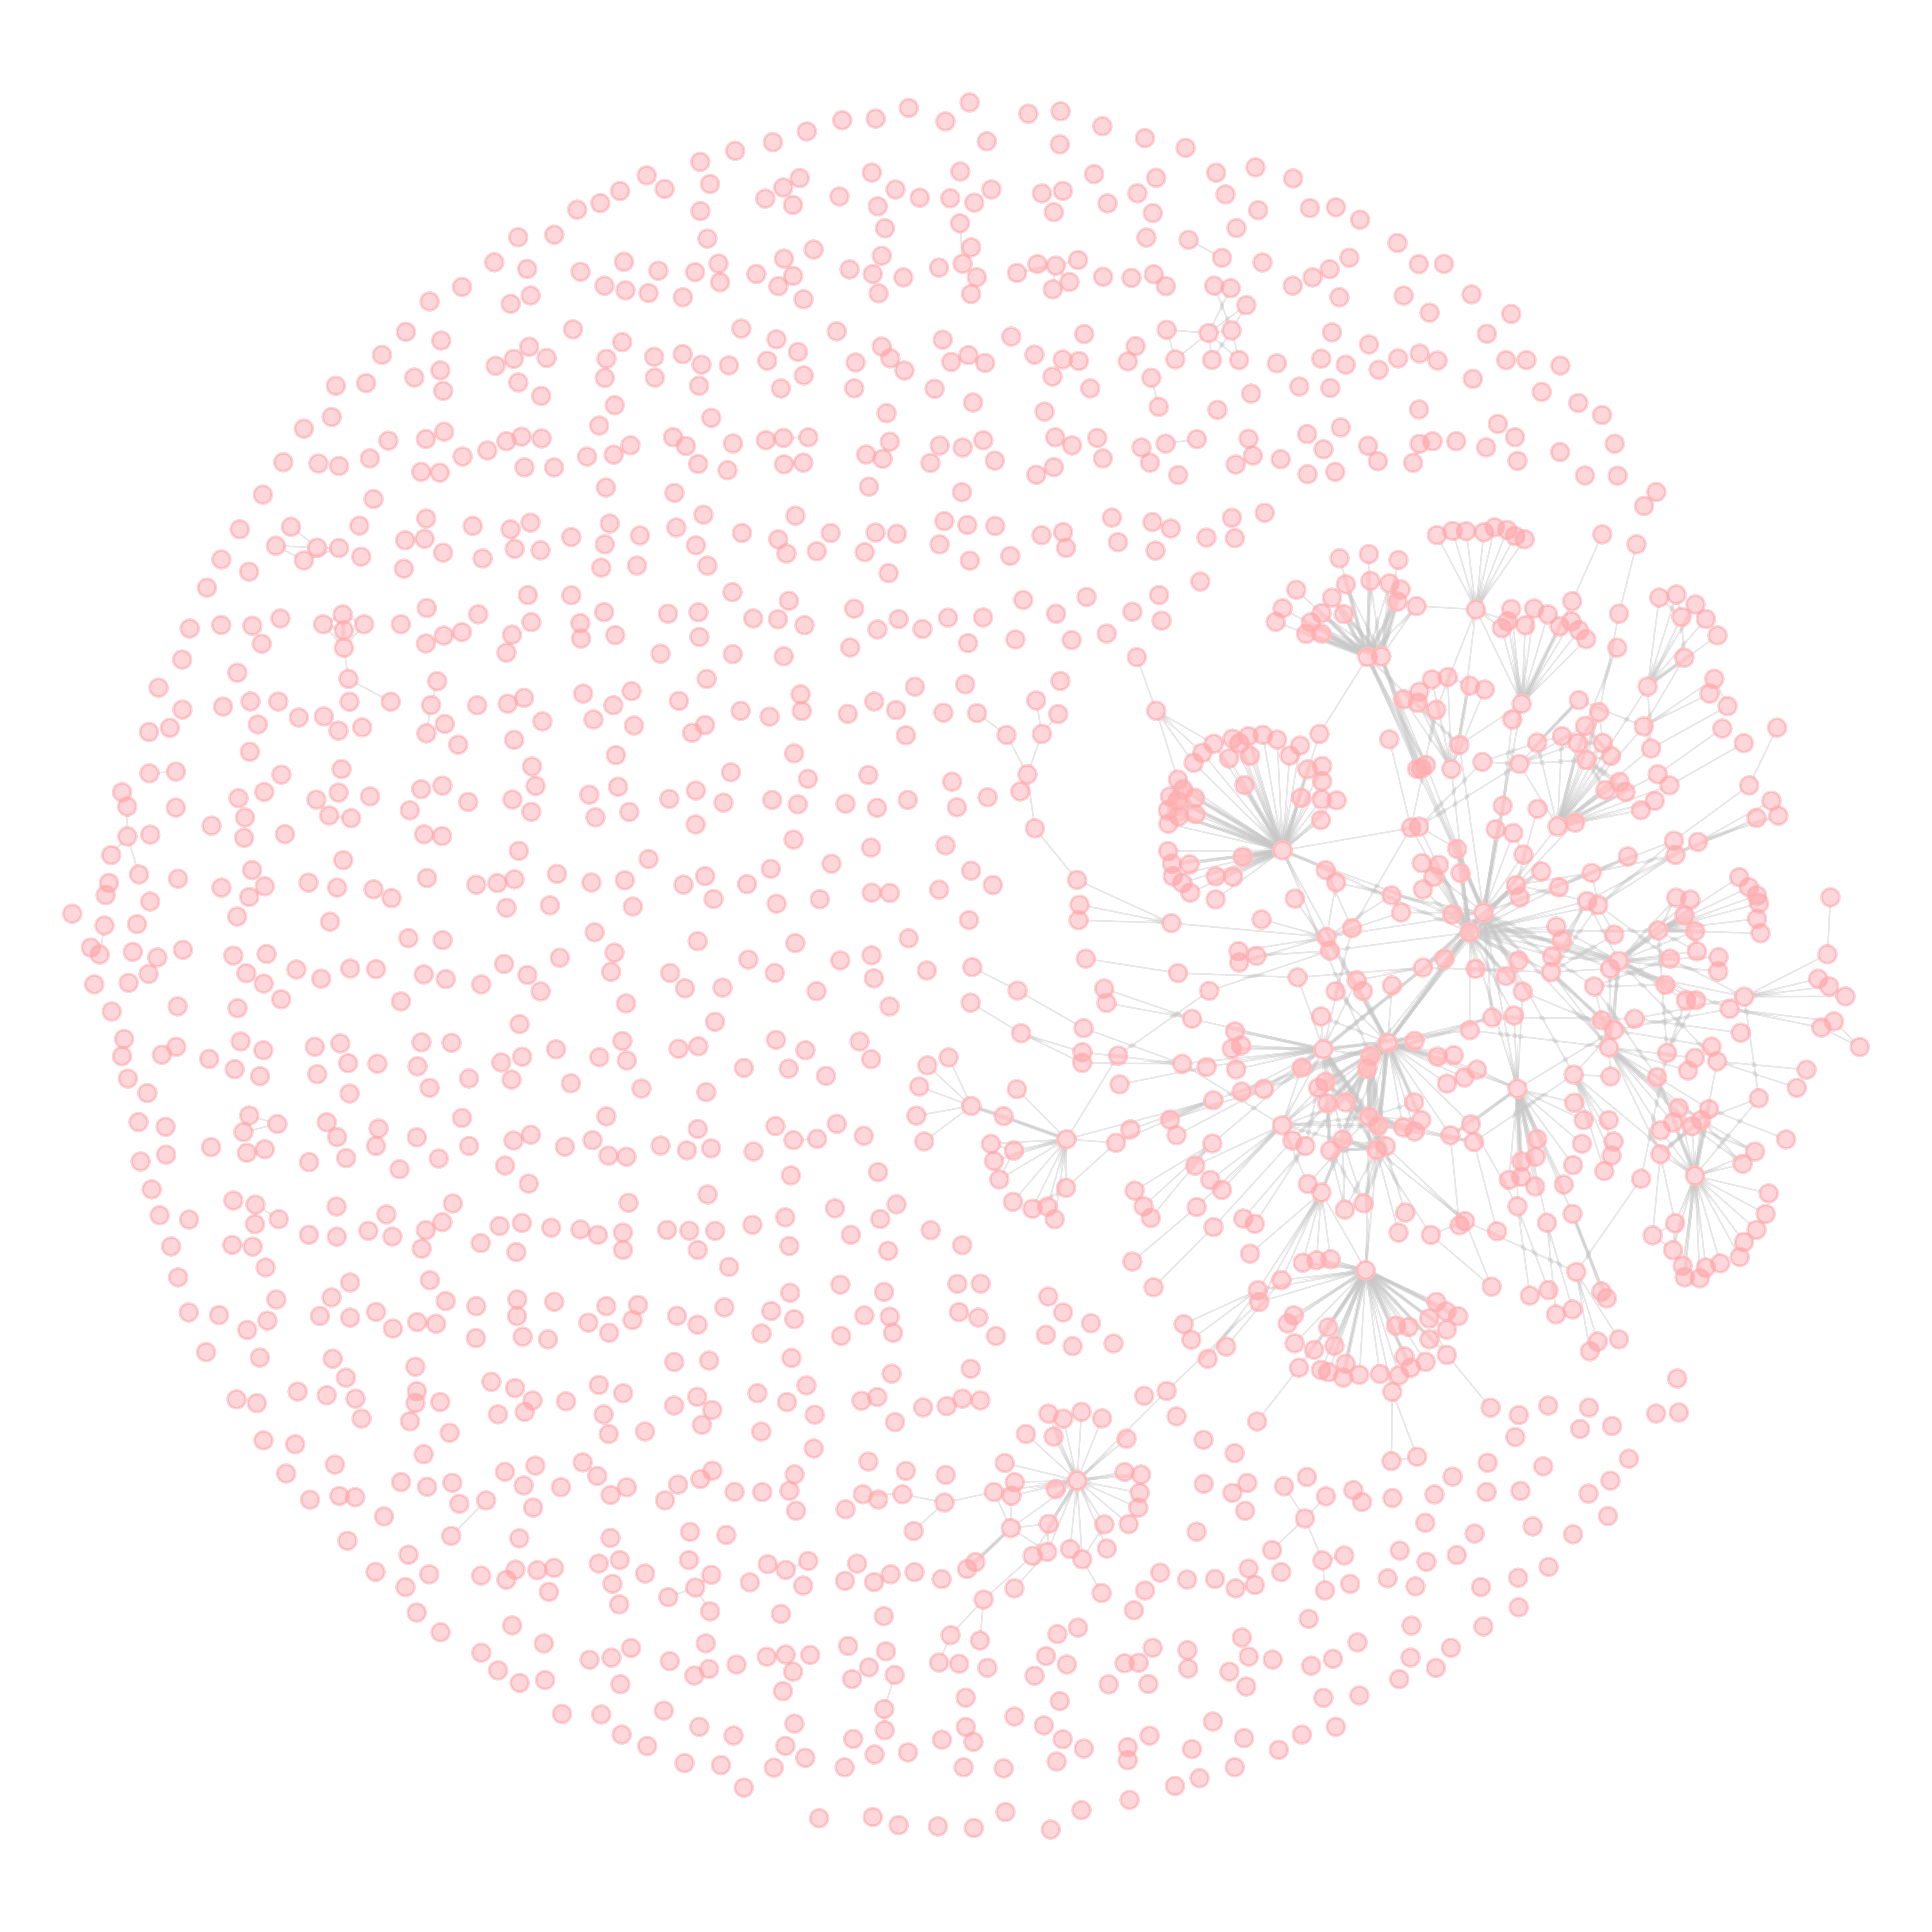
\includegraphics[width=\paperwidth]{graphics/katrinaplot.png}
\end{textblock*}

\begin{textblock*}{100mm}(20mm,0.3\textheight)
\begin{center}
\begin{itemize}
\item[\textcolor{light-gray}{\textbf{1)}}]\textcolor{light-gray}{Overview of TERGM with \& w/o vertex dynamics}
\begin{itemize}
\item[\textcolor{light-gray}{$\bullet$}] \textcolor{light-gray}{Dynamic network logistic regression w/ \& w/o vertex dynamics}
\end{itemize}
\item[\textbf{2)}] Bayesian TERGM 
\begin{itemize}
\item Bayesian analysis of DNR w/ \& w/o vertex dynamics
\end{itemize}
\item[\textbf{3)}] Empirical test cases
\begin{itemize}
\item DNC-RNC blog citation network
\item Lin Freeman's windsurfer network
\end{itemize}
\end{itemize}
\end{center}
\end{textblock*}

%----------- Fix name --------------------------------------------------%
\begin{textblock*}{100mm}(4mm,1.02\textheight)

\includegraphics[width=20mm,heighth=5mm ]{graphics/white.png}
\end{textblock*}

\begin{textblock*}{100mm}(4mm,1.02\textheight)
\emph{\tiny{\darkblue{Zack W Almquist, Sociology and Statistics, UMN}}}
\end{textblock*}
%----------- Fix name --------------------------------------------------%

\end{frame}

%----------- slide --------------------------------------------------%



%----------- reference ----------------------------------------------%
%\begin{frame}[allowframebreaks] 
%\addtocounter{framenumber}{-2}
%\addtocounter{framenumber}{-3}
%\frametitle{References}
%\def\newblock{}
%\bibliographystyle{ajs}
%\bibliography{bayesLogit}
%\end{frame}
%----------- reference ----------------------------------------------%






%%%%%%%%%%%%%%%
\begin{textblock*}{50mm}(70mm,.2\textheight)
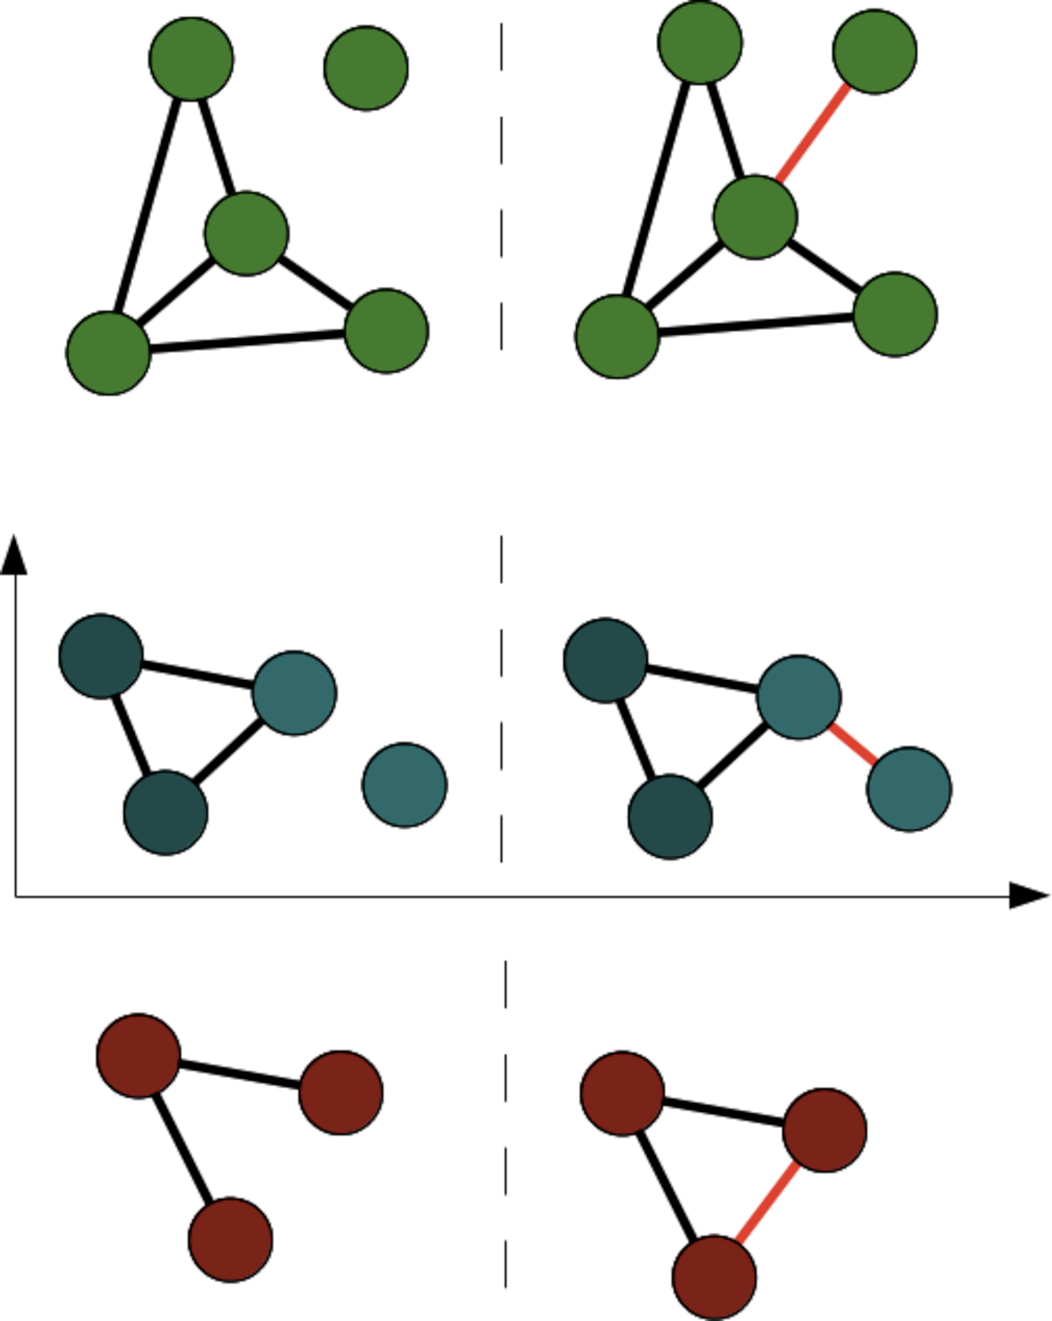
\includegraphics[width=1\linewidth]{graphics/exampleNetwork2.pdf} 
\end{textblock*}

\begin{textblock*}{60mm}(5mm,.25\textheight)
\begin{block}{Initial Intuition: Factors in Tie Formation over Time}
\begin{itemize}
\item All ties are not equally probable 
\begin{itemize}
\item Chance of an $(i,j)$ edge may depend on properties of $i$, $j$ and $t$
\item Can also depend on other $(i,j,t)$ relationships
\end{itemize}
\item Some examples:
\begin{itemize}
\item Homophily
\item Propinquity
\item Triadic/clustering effects
\begin{itemize}
\item Shared partner effects
\end{itemize}
\end{itemize}
\end{itemize}
\end{block}
\end{textblock*}
}
